
\documentclass[UTF8,12pt,openany]{ctexbook}
\usepackage[a4paper,margin=2.2cm]{geometry}
\usepackage{amsmath,amssymb,mathtools}
\usepackage{booktabs,longtable,array,multirow}
\usepackage{graphicx}
\usepackage{tikz}
\usetikzlibrary{arrows.meta,positioning,fit,shapes,calc,backgrounds}
\usepackage{enumitem}
\usepackage{xcolor}
\usepackage{listings}
\usepackage{caption}
\usepackage{float}
\usepackage{hyperref}
\usepackage{setspace}
\usepackage{fancyhdr}
\usepackage{lastpage}
\usepackage{framed}
\usepackage{tabularx}
\usepackage{makecell}
\usepackage{etoolbox}
\usepackage{titlesec}
\setstretch{1.18}
\hypersetup{colorlinks=true,linkcolor=blue!40!black,citecolor=blue!40!black,urlcolor=blue!40!black}
\pagestyle{fancy}
\fancyhf{}
\fancyhead[L]{带 Mask 的 BO3/BO5 攻防阵容 League 搜索系统}
\fancyhead[R]{\thepage}
\fancyfoot[C]{系统设计规范 v4.0}
\setlength{\headheight}{15pt}
\lstset{basicstyle=\ttfamily\small,breaklines=true,frame=single,columns=fullflexible,keepspaces=true,showstringspaces=false,tabsize=2}
\newcommand{\slot}{s}
\newcommand{\loadout}{\ell}
\newcommand{\Hcal}{\mathcal{H}}
\newcommand{\Lcal}{\mathcal{L}}
\newcommand{\Scal}{\mathcal{S}}
\newcommand{\Ccal}{\mathcal{C}}
\newcommand{\Ecal}{\mathcal{E}}
\newcommand{\Bcal}{\mathcal{B}}
\newcommand{\Qcal}{\mathcal{Q}}
\newcommand{\Legal}{\mathsf{Legal}}
\newcommand{\LegalAttack}{\mathsf{LegalAttack}}
\newcommand{\LegalDefense}{\mathsf{LegalDefense}}
\newcommand{\Observe}{\mathsf{Observe}}
\newcommand{\AttackOracle}{\mathsf{AttackOracle}}
\newcommand{\DefenseOracle}{\mathsf{DefenseOracle}}
\newcommand{\Power}{\mathsf{Power}}
\newcommand{\Cost}{\mathsf{Cost}}
\newcommand{\sigmoid}{\operatorname{sigmoid}}
\newcommand{\softmax}{\operatorname{softmax}}
\newcommand{\logit}{\operatorname{logit}}
\DeclareMathOperator*{\argmax}{arg\,max}
\newcommand{\E}{\mathbb{E}}
\newenvironment{designbox}{\begin{framed}\noindent\textbf{设计约束：}\ }{\end{framed}}
\newenvironment{implbox}{\begin{framed}\noindent\textbf{实现要求：}\ }{\end{framed}}
\title{\Huge 带 Mask 的 BO3/BO5 攻防阵容 League 搜索系统\\[6pt]\Large 问题形式化、网络架构、约束推断、下克上目标与执行规范\\[12pt]\large v4.0 详细设计文档}
\author{系统设计草案}
\date{2026-07-04}

\begin{document}

\maketitle
\thispagestyle{empty}
\clearpage
\chapter*{版本说明}
本文件是 v4.0 详细设计规范。它在上一版基础上做了四个关键升级。第一，前文和网络架构都显式使用站位信息，不再只在合法性检查阶段使用站位顺序。第二，数据结构从裸英雄升级为 position-aware loadout，唯一传奇装备星级被纳入状态、belief 和胜率模型。第三，进攻和防守都加入“下克上”目标，包括资源成本、战力差、counter residual、goal-conditioned generation 和 underdog exploiter。第四，文档不只描述思路，而是给出可执行的模块契约、网络输入输出、损失函数、候选生成流程、仿真调度和验收测试。

本文目标读者包括实现工程师、训练框架开发者、策略搜索模型、数据管线模型和评估模型。执行时应把本文视为系统规范，而不是单一模型说明。
\tableofcontents
\clearpage

\mainmatter

\chapter{核心目标与系统边界}

\section{系统要解决的问题}
本系统面向 BO3 或 BO5 的攻防阵容决策。系统需要在给定英雄池、装备池、站位顺序、唯一传奇装备互斥、普通装备可重复、mask 隐藏信息、仿真数据和真实平台数据的条件下，自动输出进攻方案或防守方案。

它不是一个简单的分类器。一个分类器的形式通常是“输入一个防守，输出一个进攻”。这个问题不能这样做，原因有三点。第一，合法输出空间非常稀疏，BO5 有 25 个英雄槽，随便输出会大量违反英雄唯一性、唯一装备唯一性和站位顺序。第二，防守被 mask 后，进攻方看到的是 observation，而不是完整阵容，必须对隐藏部分做 belief 推断。第三，真实平台上的阵容分布和仿真中的随机分布不一致，需要 sim-to-real 校准。

\section{系统的决策对象}
系统有两个主要在线决策任务。进攻任务输入对方完整防守或 mask observation，输出合法的 AttackPlan。防守任务输入当前攻击 meta 和防守方英雄资源，输出 DefensePlan，也就是真实防守 roster 与 mask 的组合。

\begin{align}
A^*(O) &= \arg\max_{A:\LegalAttack_n(A)=1}\; \mathbb{E}_{L\sim b(L|O)}[U(A,L)], \\
D^* &= (R^*,M^*) = \arg\min_{R,M:\LegalDefense_n(R,M)=1}\; U(A^*(\Observe(R,M)),R).
\end{align}

这里 $A$ 是进攻方案，$R$ 是真实防守 roster，$M$ 是 mask，$D=(R,M)$ 是完整防守策略，$O=\Observe(R,M)$ 是攻击方实际看到的信息，$L$ 是包含英雄、装备、星级、练度与站位的完整 loadout roster。

\section{系统不是一个模型，而是一个闭环}
最终系统由多个模块组成：SurrogateScorer、LegalPlanGenerator、BeliefEngine、AttackGenerationNetwork、DefenseRosterGenerationNetwork、MaskSelectionNetwork、AttackOracle、DefenseOracle、ActivePerceptionScheduler、RealCalibrationModel 和 LeagueManager。每个模块只负责一部分功能，最终输出由搜索和仿真复评确定。

\begin{figure}[H]
\centering
\resizebox{0.95\textwidth}{!}{%
\begin{tikzpicture}[node distance=1.35cm and 1.8cm,>=Latex, every node/.style={font=\small}]
\tikzstyle{box}=[draw,rounded corners,align=center,minimum width=2.8cm,minimum height=0.9cm]
\node[box,fill=blue!8] (real) {RealMetaDB\\真实平台数据库};
\node[box,fill=blue!8,below=of real] (adapter) {RealMetaAdapter\\分布重加权/校准};
\node[box,fill=green!8,below=of adapter] (belief) {BeliefEngine\\约束补全 + 概率 belief};
\node[box,fill=orange!12,left=of belief] (attack) {AttackOracle\\进攻 best response};
\node[box,fill=orange!12,right=of belief] (defense) {DefenseOracle\\防守 best response};
\node[box,fill=purple!10,left=of attack] (surrogate) {SurrogateScorer\\单队胜率 + 不确定性};
\node[box,fill=cyan!10,below=of attack] (apool) {AttackPool\\main/exploiter/history};
\node[box,fill=cyan!10,below=of defense] (dpool) {DefensePool\\roster + mask};
\node[box,fill=green!10,below right=0.6cm and -0.8cm of apool] (league) {LeagueManager\\AlphaStar-style PSRO};
\node[box,fill=red!8,below left=0.8cm and -0.2cm of apool] (sim) {Simulator Workers\\BO3/BO5 仿真};
\node[box,fill=yellow!15,right=of dpool] (active) {ActivePerception\\主动感知调度};
\draw[->] (real) -- (adapter);
\draw[->] (adapter) -- (belief);
\draw[->] (belief) -- (attack);
\draw[->] (belief) -- (defense);
\draw[->] (surrogate) -- (attack);
\draw[->] (attack) -- (apool);
\draw[->] (defense) -- (dpool);
\draw[->] (apool) -- (league);
\draw[->] (dpool) -- (league);
\draw[->] (league) -- (attack);
\draw[->] (league) -- (defense);
\draw[->] (active) -- (sim);
\draw[->] (league) -- (active);
\draw[->] (sim) -- (surrogate);
\draw[->] (sim) -- (real);
\draw[->] (real.east) .. controls +(2.6,0.0) and +(2.0,1.2) .. (active.north);
\end{tikzpicture}}
\caption{系统总架构。仿真负责探索，真实平台数据库负责校准，BeliefEngine 负责 mask 不完全信息，Attack/Defense Oracle 负责 best response，LeagueManager 负责长期攻防循环。}
\end{figure}

\section{设计原则}
\begin{enumerate}[leftmargin=2em]
\item \textbf{合法性由结构保证。} 不允许网络自由输出非法阵容再过滤。生成过程必须使用 legal action mask、forward checking 或约束求解器。
\item \textbf{模型只做 proposal 和估值。} 单队网络和生成网络不能替代仿真。最终 top 方案必须经过真实仿真或真实平台数据校准。
\item \textbf{先规则剪枝，再概率推断。} mask 后隐藏信息必须先由站位、英雄唯一、唯一装备、装备星级域等规则构造可行补全集合。
\item \textbf{目标包含下克上。} 系统不只最大化胜率，也要显式学习低资源反制高资源的策略。
\item \textbf{League 防止局部过拟合。} 维护 main、exploiter、historical、underdog 策略池，避免只适配当前单一 meta。
\end{enumerate}


\chapter{问题形式化：符号、对象与数据结构}

\section{MatchFormat}
比赛格式定义为
\begin{equation}
F=(n,m,r,c_{hide},C_{hide}),
\end{equation}
其中 $n$ 是队伍数量，$m=5$ 是每队英雄数，$r=\lfloor n/2\rfloor+1$ 是获胜需要赢下的小局数，$c_{hide}=2$ 是每队最多隐藏位置数，$C_{hide}=10$ 是全局最多隐藏位置数。BO3 时 $n=3,r=2$；BO5 时 $n=5,r=3$。

槽位集合定义为
\begin{equation}
\Scal_n=\{(i,j): i=1,\ldots,n,\; j=1,\ldots,5\}.
\end{equation}
$(i,j)$ 表示第 $i$ 队第 $j$ 个站位槽。

\begin{lstlisting}[caption={MatchFormat 数据结构}]
@dataclass(frozen=True)
class MatchFormat:
    n_teams: int                  # 3 for BO3, 5 for BO5
    team_size: int = 5
    win_required: int | None = None
    max_hidden_per_team: int = 2
    max_hidden_total: int = 10

    def __post_init__(self):
        if self.win_required is None:
            object.__setattr__(self, "win_required", self.n_teams // 2 + 1)
        assert self.n_teams in (3, 5)
        assert self.team_size == 5
\end{lstlisting}

\section{HeroRecord 与 Loadout}
英雄全集记为 $\Hcal$。攻击方可用 loadout 集合记为 $\Lcal_A$，防守方可用 loadout 集合记为 $\Lcal_D$。工程实现中所有生成动作都应以 loadout 为单位，而不是裸英雄。一个 loadout 定义为
\begin{equation}
\ell=(h,u,s^u,g,x,\rho),
\end{equation}
其中 $h$ 是英雄 ID，$u$ 是唯一传奇装备 ID，$s^u\in\{3,4,5\}$ 是唯一传奇装备星级，$g$ 是普通装备配置，$x$ 是练度和属性特征，$\rho$ 是站位秩。

唯一性约束默认作用在唯一装备 ID 上，而不是星级上。也就是说，如果两个 loadout 使用同一个唯一传奇装备 ID，即使星级不同，也视为冲突。

\begin{lstlisting}[caption={HeroRecord 与 Loadout 数据结构}]
@dataclass(frozen=True)
class HeroRecord:
    hero_id: int
    name: str
    standing_rank: float
    standing_bucket: str          # front / mid / back / custom
    role_tags: tuple[str, ...]
    base_stats: dict[str, float]
    base_power: float
    default_unique_equip_id: int | None

@dataclass(frozen=True)
class Loadout:
    hero_id: int
    unique_equip_id: int | None
    unique_equip_star: int | None # 3, 4, 5; None if no unique equip
    normal_equip_ids: tuple[int, ...]
    normal_equip_features: dict[str, float]
    level_features: dict[str, float]
    final_stats: dict[str, float]
    final_power: float
    standing_rank: float
    standing_bucket: str
\end{lstlisting}

\section{站位顺序}
每个 loadout 有站位秩 $\rho(\ell)\in\mathbb{R}$。一队从前到后必须满足
\begin{equation}
\rho(T_{i,1}) < \rho(T_{i,2}) < \cdots < \rho(T_{i,5}).
\end{equation}
站位不只是合法性条件，也是网络输入特征。它会影响受击顺序、保护关系、切后目标、技能范围和隐藏补全可行域。

\section{AttackPlan}
进攻方案是一个从槽位到 loadout 的赋值函数：
\begin{equation}
A:\Scal_n\rightarrow \Lcal_A.
\end{equation}
写作 $A_{i,j}=A(i,j)$。第 $i$ 队为
\begin{equation}
A_i=(A_{i,1},A_{i,2},A_{i,3},A_{i,4},A_{i,5}).
\end{equation}
完整进攻方案为
\begin{equation}
A=(A_1,A_2,\ldots,A_n).
\end{equation}

合法性谓词 $\LegalAttack_n(A)=1$ 要求：所有 loadout 来自攻击方可用集合；英雄 ID 全局不重复；非空唯一装备 ID 全局不重复；每队站位严格递增。

\begin{lstlisting}[caption={AttackPlan 数据结构}]
@dataclass(frozen=True)
class Team:
    slots: tuple[Loadout, ...]    # length 5, ordered by standing position

@dataclass(frozen=True)
class AttackPlan:
    format: MatchFormat
    teams: tuple[Team, ...]       # length n_teams
    source: str                   # random/search/main/exploiter/real
    plan_id: str | None = None
\end{lstlisting}

\section{DefenseRoster、Mask 与 DefensePlan}
真实防守 roster 是
\begin{equation}
R:\Scal_n\rightarrow \Lcal_D.
\end{equation}
mask 是二值函数
\begin{equation}
M:\Scal_n\rightarrow\{0,1\}.
\end{equation}
$M_{i,j}=1$ 表示隐藏，$M_{i,j}=0$ 表示可见。完整防守方案是
\begin{equation}
D=(R,M).
\end{equation}

防守合法性除了 roster 的英雄、装备、站位约束，还包括 mask 约束：
\begin{align}
\sum_{j=1}^{5}M_{i,j} &\le c_{hide},\quad \forall i,\\
\sum_{i=1}^{n}\sum_{j=1}^{5}M_{i,j} &\le C_{hide}.
\end{align}

\begin{lstlisting}[caption={DefensePlan 数据结构}]
@dataclass(frozen=True)
class DefensePlan:
    format: MatchFormat
    teams: tuple[Team, ...]       # real roster R
    mask: tuple[tuple[int, ...], ...]  # n_teams x 5
    source: str
    plan_id: str | None = None
\end{lstlisting}

\section{Observation}
攻击方看到的 observation 由完整防守和 mask 生成：
\begin{equation}
O=\Observe(R,M).
\end{equation}
对每个槽位：
\begin{equation}
O_{i,j}=\begin{cases}
R_{i,j}, & M_{i,j}=0,\\
\bot, & M_{i,j}=1.
\end{cases}
\end{equation}
如果可见槽位包含装备信息，则 observation 中应包括英雄 ID、唯一装备 ID、唯一装备星级、普通装备摘要、战力摘要和站位秩。如果隐藏，则这些字段为 unknown。

\begin{lstlisting}[caption={Observation 数据结构}]
@dataclass(frozen=True)
class VisibleSlot:
    hero_id: int | None
    unique_equip_id: int | None
    unique_equip_star: int | None
    normal_equip_summary: tuple[int, ...] | None
    final_power: float | None
    standing_rank: float | None
    is_hidden: bool

@dataclass(frozen=True)
class Observation:
    format: MatchFormat
    slots: tuple[tuple[VisibleSlot, ...], ...]
    hidden_slots: tuple[tuple[int, int], ...]
    visible_heroes: frozenset[int]
    visible_unique_equip_ids: frozenset[int]
    visible_unique_equip_stars: dict[int, int]
\end{lstlisting}

\begin{figure}[H]
\centering
\resizebox{0.92\textwidth}{!}{%
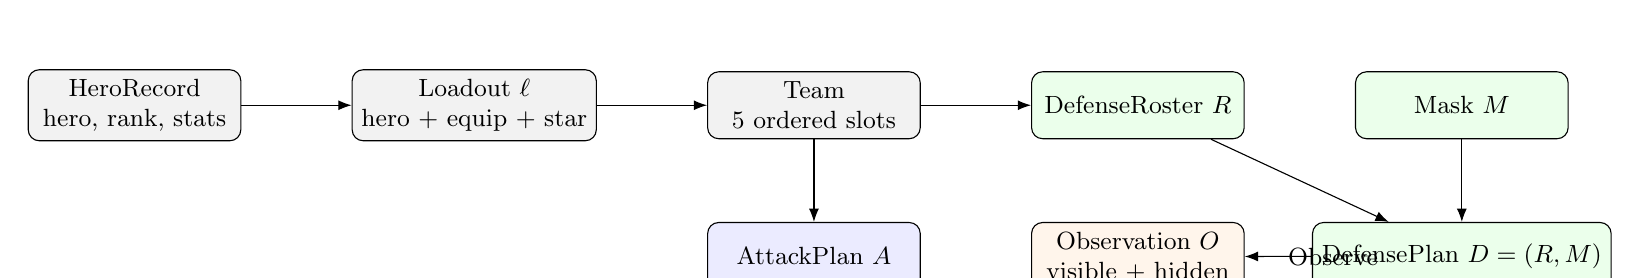
\begin{tikzpicture}[node distance=1.05cm and 1.4cm,>=Latex, every node/.style={font=\small}]
\tikzstyle{box}=[draw,rounded corners,align=center,minimum width=2.7cm,minimum height=0.85cm]
\node[box,fill=gray!10] (hero) {HeroRecord\\hero, rank, stats};
\node[box,fill=gray!10,right=of hero] (loadout) {Loadout $\ell$\\hero + equip + star};
\node[box,fill=gray!10,right=of loadout] (team) {Team\\5 ordered slots};
\node[box,fill=blue!8,below=of team] (attack) {AttackPlan $A$};
\node[box,fill=green!8,right=of team] (roster) {DefenseRoster $R$};
\node[box,fill=green!8,right=of roster] (mask) {Mask $M$};
\node[box,fill=green!8,below=of mask] (defplan) {DefensePlan $D=(R,M)$};
\node[box,fill=orange!8,below=of roster] (obs) {Observation $O$\\visible + hidden};
\draw[->] (hero) -- (loadout);
\draw[->] (loadout) -- (team);
\draw[->] (team) -- (attack);
\draw[->] (team) -- (roster);
\draw[->] (roster) -- (defplan);
\draw[->] (mask) -- (defplan);
\draw[->] (defplan) -- node[right]{Observe} (obs);
\end{tikzpicture}}
\caption{核心数据对象。工程实现中基本动作对象是 Loadout，而不是裸英雄。Loadout 包含唯一传奇装备 ID、装备星级、普通装备、练度和站位特征。}
\end{figure}

\section{核心符号表}
\begin{longtable}{p{0.20\linewidth}p{0.73\linewidth}}
\toprule
符号 & 含义 \\
\midrule
$F$ & MatchFormat，包含队伍数量、获胜局数和 mask 限制。\\
$n$ & 队伍数量，BO3 为 3，BO5 为 5。\\
$r$ & 获胜所需小局数，$r=\lfloor n/2\rfloor+1$。\\
$\Scal_n$ & 所有槽位集合，元素为 $(i,j)$。\\
$\Hcal$ & 英雄全集。\\
$\Lcal_A,\Lcal_D$ & 攻击方、防守方可用 loadout 集合。\\
$\ell$ & 一个 hero-loadout，包含英雄、装备、星级、普通装备、属性、站位。\\
$u(\ell)$ & loadout 使用的唯一传奇装备 ID。\\
$s^u(\ell)$ & 唯一传奇装备星级，取值 3、4、5。\\
$\rho(\ell)$ & 站位秩。\\
$A$ & AttackPlan，进攻方完整 N 队方案。\\
$R$ & DefenseRoster，防守方真实完整 roster，不含 mask。\\
$M$ & Mask，二值隐藏函数。\\
$D=(R,M)$ & DefensePlan，完整防守策略。\\
$O$ & Observation，攻击方看到的信息。\\
$\Ccal_L(O)$ & 兼容 observation 的可行 loadout 补全集合。\\
$b(L|O)$ & 在可行补全集合上的 belief 分布。\\
$U(A,L)$ & 进攻方案对完整防守 loadout roster 的 match 胜率。\\
\bottomrule
\end{longtable}


\chapter{约束系统：站位、英雄唯一、装备星级与可行补全}

\section{为什么约束系统必须独立成模块}
mask 下隐藏阵容推断不能直接交给神经网络。神经网络可以给概率，但不能承担硬规则。正确顺序是：先构造每个隐藏槽位的候选域，再用 forward checking 或 beam search 枚举可行补全，最后在这些补全上做概率 belief。

\section{隐藏槽位候选域}
对隐藏槽位 $s=(i,j)$，候选域记为 $\Omega_s(O)\subseteq\Lcal_D$。它由站位、英雄唯一性、唯一装备 ID、装备星级域和可用池共同决定。

站位边界定义为：
\begin{align}
L_{i,j}(O)&=\max_{k<j,\;O_{i,k}\ne\bot}\rho(O_{i,k}),\\
U_{i,j}(O)&=\min_{k>j,\;O_{i,k}\ne\bot}\rho(O_{i,k}).
\end{align}
如果左侧没有可见英雄，用 $-\infty$；如果右侧没有可见英雄，用 $+\infty$。

站位候选域为：
\begin{equation}
\Omega^{pos}_{i,j}(O)=\{\ell\in\Lcal_D: L_{i,j}(O)<\rho(\ell)<U_{i,j}(O)\}.
\end{equation}

\section{英雄唯一性与唯一装备 ID}
可见英雄集合为 $H_{vis}(O)$。可见唯一装备 ID 集合为 $E^u_{vis}(O)$。候选 loadout 必须满足
\begin{align}
h(\ell)&\notin H_{vis}(O),\\
u(\ell)&\notin E^u_{vis}(O)\quad \text{if }u(\ell)\ne\varnothing.
\end{align}
隐藏槽位之间也要满足 AllDifferent 约束：
\begin{align}
h(\ell_s)&\ne h(\ell_t),\quad s\ne t,\\
u(\ell_s)&\ne u(\ell_t),\quad s\ne t,
\end{align}
其中唯一装备为空时不产生冲突。

\section{唯一传奇装备星级}
唯一传奇装备星级 $s^u\in\{3,4,5\}$ 是状态的一部分。它影响强度、belief 和下克上潜力，但默认不影响唯一性 key。也就是说，唯一性按装备 ID 判断：同一个装备 ID 即使星级不同也冲突。

如果敌方隐藏位的装备星级不可见，则 belief 应在星级上边缘化：
\begin{equation}
b(L|O)=P(L|O),\quad L=(\ell_s)_{s\in\Scal_n}.
\end{equation}
如果缺少真实统计，初版可使用先验 $P(s^u=3)=P(s^u=4)=P(s^u=5)=1/3$。后期应由 RealMetaDB 学习
\begin{equation}
P(s^u|h,u,O,\text{season},\text{rank segment}).
\end{equation}

\section{可行补全集合}
完整可行 loadout 补全集合为：
\begin{equation}
\Ccal_L(O)=\{L: L_s=O_s\ \forall s\in\mathcal{V}(O),\; L_s\in\Omega_s(O)\ \forall s\in\mathcal{Z}(O),\; \LegalDefense_n(L,M)=1\}.
\end{equation}
这里 $\mathcal{V}(O)$ 是可见槽位集合，$\mathcal{Z}(O)$ 是隐藏槽位集合。

\section{Forward Checking 与 MRV}
隐藏位之间不是独立分类任务。每选择一个隐藏 loadout，都要从其他隐藏域删除同英雄和同唯一装备 ID 的候选。因此补全应使用约束满足问题的做法。

\begin{lstlisting}[caption={隐藏补全的约束传播伪代码}]
def complete_hidden_slots(observation, domains):
    assignments = {}
    return backtrack(assignments, domains)

def backtrack(assignments, domains):
    if all_slots_assigned(assignments, domains):
        return [assignments]

    slot = select_mrv_slot(domains, assignments)
    results = []
    for loadout in order_by_belief_score(domains[slot]):
        if violates_global_constraints(loadout, assignments):
            continue
        new_domains = forward_check(domains, slot, loadout)
        if any_empty_domain(new_domains):
            continue
        results.extend(backtrack(assignments | {slot: loadout}, new_domains))
    return results
\end{lstlisting}

\begin{figure}[H]
\centering
\resizebox{!}{0.72\textheight}{%
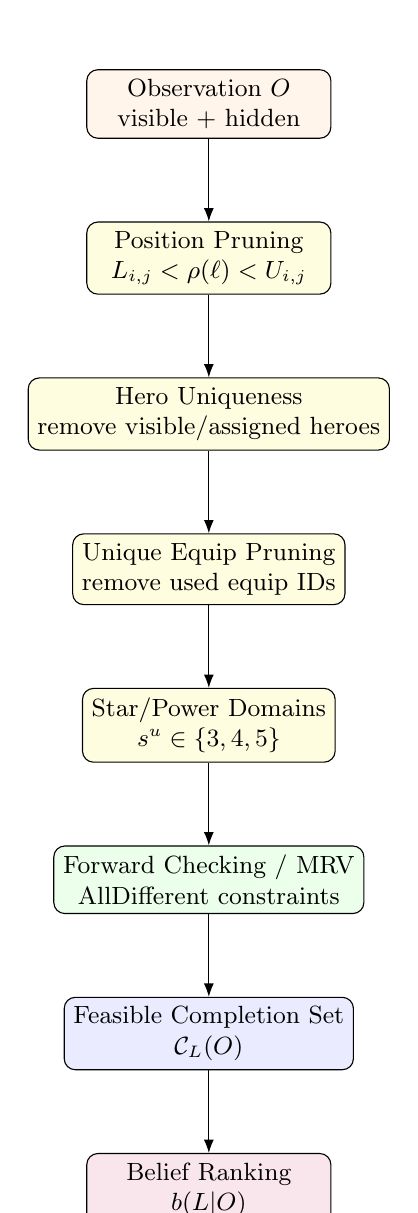
\begin{tikzpicture}[node distance=1.05cm and 1.3cm,>=Latex, every node/.style={font=\small}]
\tikzstyle{box}=[draw,rounded corners,align=center,minimum width=3.1cm,minimum height=0.85cm]
\node[box,fill=orange!8] (obs) {Observation $O$\\visible + hidden};
\node[box,fill=yellow!12,below=of obs] (pos) {Position Pruning\\$L_{i,j}<\rho(\ell)<U_{i,j}$};
\node[box,fill=yellow!12,below=of pos] (hero) {Hero Uniqueness\\remove visible/assigned heroes};
\node[box,fill=yellow!12,below=of hero] (equip) {Unique Equip Pruning\\remove used equip IDs};
\node[box,fill=yellow!12,below=of equip] (star) {Star/Power Domains\\$s^u\in\{3,4,5\}$};
\node[box,fill=green!8,below=of star] (mrv) {Forward Checking / MRV\\AllDifferent constraints};
\node[box,fill=blue!8,below=of mrv] (cand) {Feasible Completion Set\\$\mathcal{C}_L(O)$};
\node[box,fill=purple!10,below=of cand] (belief) {Belief Ranking\\$b(L|O)$};
\draw[->] (obs) -- (pos);
\draw[->] (pos) -- (hero);
\draw[->] (hero) -- (equip);
\draw[->] (equip) -- (star);
\draw[->] (star) -- (mrv);
\draw[->] (mrv) -- (cand);
\draw[->] (cand) -- (belief);
\end{tikzpicture}}
\caption{BeliefEngine 的正确顺序。先用站位、英雄、唯一装备和星级域进行硬剪枝，再对可行补全做概率打分。}
\end{figure}

\section{模块契约}
ConstraintEngine 必须暴露以下接口：
\begin{lstlisting}[caption={ConstraintEngine 接口}]
class ConstraintEngine:
    def build_domains(self, observation: Observation) -> dict[Slot, list[Loadout]]: ...
    def is_legal_attack(self, plan: AttackPlan) -> bool: ...
    def is_legal_defense(self, plan: DefensePlan) -> bool: ...
    def enumerate_completions(self, observation: Observation, max_k: int) -> list[DefenseRoster]: ...
    def beam_complete(self, observation: Observation, beam_size: int, max_k: int) -> list[DefenseRoster]: ...
\end{lstlisting}

验收标准是：任何来自 ConstraintEngine 的补全都必须满足站位严格递增、英雄不重复、唯一装备 ID 不重复、可见槽位一致和 mask 约束。任何不满足这些条件的输出都应视为系统错误，而不是低质量预测。


\chapter{效用函数：BO3/BO5 胜率、资源成本与下克上目标}

\section{单路胜率到整体胜率}
单路胜率由 SingleTeamWinrateModel 输出：
\begin{equation}
f_\theta(A_i,L_i)=(\mu_i,\sigma_i,\hat m_i,\hat t_i).
\end{equation}
其中 $\mu_i$ 是胜率均值，$\sigma_i$ 是不确定性，$\hat m_i$ 是 margin，$\hat t_i$ 是战斗时长。

保守胜率：
\begin{equation}
\tilde p_i=\mathrm{clip}(\mu_i-\beta\sigma_i,\epsilon,1-\epsilon).
\end{equation}
探索胜率：
\begin{equation}
p_i^{ucb}=\mathrm{clip}(\mu_i+\beta\sigma_i,\epsilon,1-\epsilon).
\end{equation}

整体 match 胜率定义为：
\begin{equation}
U(A,L)=P\left(\sum_{i=1}^{n}X_i\ge r\right),\quad X_i\sim\mathrm{Bernoulli}(p_i).
\end{equation}
动态规划统一计算 BO3 和 BO5：
\begin{align}
dp_0[0]&=1,\\
dp_i[w]&=dp_{i-1}[w](1-p_i)+dp_{i-1}[w-1]p_i,\\
U(A,L)&=\sum_{w=r}^{n}dp_n[w].
\end{align}

\section{资源成本}
为了实现下克上，需要定义资源成本。一个 loadout 的成本可以写成
\begin{equation}
C(\ell)=\alpha_p\Power(\ell)+\alpha_s StarCost(s^u(\ell))+\alpha_r RareHeroCost(h(\ell))+\alpha_g GearCost(g(\ell)).
\end{equation}
一个 plan 的成本为
\begin{equation}
C(A)=\sum_{\ell\in A}C(\ell),\quad C(L)=\sum_{\ell\in L}C(\ell).
\end{equation}

\section{进攻下克上}
进攻下克上表示进攻资源低于防守资源但仍能赢。定义
\begin{equation}
Gap_A(A,L)=\frac{C(L)-C(A)}{C(L)+\epsilon}.
\end{equation}
当 $Gap_A>0$ 时，进攻方资源更低。

进攻目标可写为：
\begin{equation}
J_A(A|O)=\E_{L\sim b(L|O)}[U(A,L)]+\lambda_u\E_{L\sim b(L|O)}[\max(0,Gap_A(A,L))]-\lambda_c C(A).
\end{equation}
也可以使用约束式：
\begin{equation}
\max_A\E_{L\sim b(L|O)}[U(A,L)]\quad \text{s.t.}\quad C(A)\le \tau\E_{L\sim b(L|O)}[C(L)].
\end{equation}

\section{防守下克上}
防守下克上表示防守方用较低资源抵抗更高资源进攻。定义
\begin{equation}
Gap_D(A,L)=\frac{C(A)-C(L)}{C(A)+\epsilon}.
\end{equation}
防守目标：
\begin{equation}
\begin{aligned}
J_D(L,M)=&-\E_{A\sim\sigma_A}[U(A,L)]
+\lambda_u\E_{A\sim\sigma_A}[\max(0,Gap_D(A,L))]\\
&+\lambda_m \mathrm{Ambiguity}(\Observe(L,M))-\lambda_c C(L).
\end{aligned}
\end{equation}

\section{Power Residual Modeling}
如果直接训练胜率模型，模型容易学到“战力高的一方赢”。为了发现下克上，应把数值优势和克制残差分开：
\begin{equation}
\logit(p)=Baseline(\Delta Power,\Delta Star)+CounterResidual_\theta(A_i,L_i).
\end{equation}
其中
\begin{equation}
\Delta Power=C(A_i)-C(L_i),\quad \Delta Star=\overline{s^u_A}-\overline{s^u_L}.
\end{equation}
Baseline 解释纯属性碾压，CounterResidual 学习克制、站位、技能协同和装备配置带来的额外胜率。

\begin{implbox}
任何生成网络、搜索器和 active sampler 都必须显式保留 underdog 模式。实现上至少支持三个 goal 参数：\texttt{target\_power\_ratio=1.0}、\texttt{0.9}、\texttt{0.8}。它们分别表示平等资源、低 10\% 资源和低 20\% 资源下的进攻或防守搜索。
\end{implbox}


\chapter{Position-aware SingleTeamWinrateModel}

\section{任务定义}
SingleTeamWinrateModel 输入一个进攻单队和一个防守单队，输出胜率、不确定性、margin 和战斗时长。它是整个系统的 learned surrogate。它不能替代仿真，但必须足够好地排序候选并指出不确定区域。

输入：
\begin{equation}
(A_i,L_i)=((\ell^A_{i,1},\ldots,\ell^A_{i,5}),(\ell^D_{i,1},\ldots,\ell^D_{i,5})).
\end{equation}
输出：
\begin{equation}
(\mu,\sigma,\hat m,\hat t,\hat r)=f_\theta(A_i,L_i),
\end{equation}
其中 $\hat r$ 是 counter residual。

\section{Loadout Encoder}
每个 loadout 编码为：
\begin{equation}
e_\ell=Emb_h(h)+Emb_u(u)+Emb_s(s^u)+Emb_b(bucket(\rho))+MLP([x,\Power,\rho]).
\end{equation}
推荐默认维度：
\begin{longtable}{p{0.34\linewidth}p{0.20\linewidth}p{0.38\linewidth}}
\toprule
组件 & 维度 & 说明 \\
\midrule
hero embedding & 128 & 英雄身份和技能隐变量。\\
unique equip embedding & 32 & 唯一传奇装备 ID。\\
unique equip star embedding & 16 & 3、4、5 星。\\
standing bucket embedding & 16 & 前排、中排、后排等离散站位。\\
stats/power MLP & 64 & 连续属性、战力、练度。\\
final loadout vector & 256 & 投影后的统一表示。\\
\bottomrule
\end{longtable}

\section{OrderedTeamEncoder}
由于站位顺序影响战斗，TeamEncoder 不应只使用 DeepSets。推荐使用 ordered Transformer：
\begin{equation}
x_{j}=e_{\ell_j}+Emb_{slot}(j)+MLP([\rho(\ell_j),j]).
\end{equation}
然后
\begin{equation}
Z_T=TransformerEncoder(x_1,\ldots,x_5).
\end{equation}
这里不使用 causal attention，因为胜率评估看到完整队伍。Transformer 内部应加入 relative position bias：
\begin{equation}
B_{jk}=Emb_{rel}(j-k)+MLP([\rho(\ell_j)-\rho(\ell_k),|\rho(\ell_j)-\rho(\ell_k)|]).
\end{equation}
注意力 logits 为
\begin{equation}
\frac{QK^\top}{\sqrt d}+B.
\end{equation}

\section{Position-aware Cross Interaction}
攻击英雄与防守英雄之间的 5x5 交互是建模克制的关键。对攻击位置 $j$ 和防守位置 $k$：
\begin{equation}
c_{jk}=\psi([e^A_j,e^D_k,e^A_j\odot e^D_k,e^A_j-e^D_k,Emb(j),Emb(k),\Delta\rho_{jk},|\Delta\rho_{jk}|,\Delta s^u_{jk},\Delta Power_{jk}]).
\end{equation}
其中 $\Delta\rho_{jk}=\rho(e^A_j)-\rho(e^D_k)$，$\Delta s^u_{jk}=s^u(e^A_j)-s^u(e^D_k)$。

池化：
\begin{equation}
z_{cross}=MeanPool(c_{jk})\;||\;MaxPool(c_{jk})\;||\;AttentionPool(c_{jk}).
\end{equation}

\section{输出头}
融合表示：
\begin{equation}
z=[z_A,z_D,z_A-z_D,z_A\odot z_D,z_{cross},\Delta Power,\Delta Star].
\end{equation}
输出：
\begin{align}
\mu&=\sigmoid(MLP_{win}(z)),\\
\sigma_{ale}&=softplus(MLP_{var}(z)),\\
\hat m&=MLP_{margin}(z),\\
\hat t&=softplus(MLP_{time}(z)),\\
\hat r&=MLP_{residual}(z).
\end{align}

\section{Ensemble 不确定性}
训练 $K$ 个模型，得到 $p_1,\ldots,p_K$。预测均值和 epistemic uncertainty：
\begin{align}
\bar p&=\frac{1}{K}\sum_{k=1}^{K}p_k,\\
\sigma^2_{epi}&=\frac{1}{K}\sum_{k=1}^{K}(p_k-\bar p)^2,\\
\sigma^2_{total}&=\sigma^2_{epi}+\sigma^2_{ale}.
\end{align}

\section{Loss}
如果一个 matchup 打 $m$ 场，赢 $w$ 场，使用 binomial NLL：
\begin{equation}
\mathcal{L}_{binom}= -[w\log\mu+(m-w)\log(1-\mu)].
\end{equation}
总损失：
\begin{equation}
\mathcal{L}=\mathcal{L}_{binom}+\lambda_m\mathcal{L}_{margin}+\lambda_t\mathcal{L}_{time}+\lambda_r\mathcal{L}_{residual}+\lambda_c\mathcal{L}_{calibration}.
\end{equation}

\section{校准指标}
Brier score：
\begin{equation}
Brier=\frac{1}{N}\sum_i(\mu_i-y_i)^2.
\end{equation}
ECE：
\begin{equation}
ECE=\sum_b\frac{|S_b|}{N}|acc(S_b)-conf(S_b)|.
\end{equation}
当模型排序好但概率不准时，应使用 temperature scaling、Platt scaling 或 isotonic regression 进行校准。


\chapter{策略生成网络通用规范：Causal Decoder、Action Mask 与 Proposal Distillation}

\section{为什么生成端必须 causal}
攻击和防守 roster 都是自回归生成序列。对于 $T=5n$ 个槽位，攻击生成分解为
\begin{equation}
P_\theta(A|O,g)=\prod_{t=1}^{T}P_\theta(a_t|O,g,a_{<t}).
\end{equation}
第 $t$ 步只能看 $a_{<t}$，不能看未来 $a_{t+1:T}$。因此 decoder self-attention 必须使用 causal mask。否则训练时会偷看未来英雄，导致 teacher-forcing loss 很低但推理时崩溃。

\section{感知端不应 causal}
ObservationEncoder、AttackMetaEncoder、SingleTeamWinrateModel、PlanEncoder 都处理已经完整可见的上下文，因此应使用 non-causal attention 或 set attention。原则是：生成端 causal，感知端 non-causal。

\section{Action Mask 与 Causal Mask 的区别}
Causal mask 解决不能看未来的问题：
\begin{equation}
C_{t,k}=\begin{cases}0,&k\le t,\\-\infty,&k>t.\end{cases}
\end{equation}
Legal action mask 解决不能选择非法 loadout 的问题：
\begin{equation}
\tilde{logit}_t(\ell)=\begin{cases}logit_t(\ell),&\ell\in Legal_t,\\-\infty,&\ell\notin Legal_t.\end{cases}
\end{equation}
最终动作分布：
\begin{equation}
P(a_t=\ell)=\softmax(\tilde{logit}_t(\ell)).
\end{equation}

\section{Legal 集合}
一个候选 loadout $\ell$ 在第 $t$ 个槽位合法，当且仅当：
\begin{enumerate}[leftmargin=2em]
\item 英雄未被选过：$h(\ell)\notin H_{selected}$。
\item 唯一装备 ID 未冲突：$u(\ell)\notin E^u_{used}$。
\item 站位顺序合法：$\rho(\ell)$ 大于当前队伍前一个槽位的站位秩。
\item 当前 slot 允许该站位 bucket。
\item 未来仍可补齐：FutureFeasible 为真。
\item 如果处于 underdog budget 模式，则选择该 loadout 后仍满足预算可行性。
\end{enumerate}

\section{FutureFeasible}
如果当前队伍还剩 $q$ 个槽位，那么选择 $\ell$ 后，剩余合法候选中必须至少有 $q$ 个站位秩更大的 loadout，并且它们之间可满足英雄和装备唯一性。这个检查可以是精确匹配，也可以用保守近似。

\section{Search Distillation}
第一阶段不建议直接训练生成网络。更稳的做法是先用合法随机、mutation、crossover、surrogate 和仿真形成 Oracle，再把 Oracle 的 top 方案蒸馏到生成网络。

对一个 observation $O$ 和搜索得到的最优方案 $A^*$：
\begin{equation}
\mathcal{L}_{BC}=-\sum_{t=1}^{T}\log P_\theta(a_t^*|O,a_{<t}^*).
\end{equation}
如果有多个候选 $A^k$，权重由仿真胜率 $v_k$ 给出：
\begin{equation}
\omega_k=\frac{\exp(v_k/\tau)}{\sum_j\exp(v_j/\tau)}.
\end{equation}

\section{生成网络在系统中的角色}
生成网络不是最终裁判。它只是 proposal generator。最终流程是：生成网络提出候选，SurrogateScorer 快速估值，约束和多样性选择筛选，仿真复评确定最终输出。


\chapter{AttackGenerationNetwork：进攻候选生成网络}

\section{任务定义}
AttackGenerationNetwork 输入 observation、belief、攻击方 loadout pool、当前生成状态和目标条件，输出合法 AttackPlan 候选。它可以用于完整信息攻击，也可以用于 mask observation 攻击。

\section{输入}
\begin{lstlisting}[caption={AttackNetInput}]
@dataclass(frozen=True)
class AttackNetInput:
    format: MatchFormat
    observation: Observation
    belief_topk: tuple[tuple[DefenseRoster, float], ...]
    attack_loadout_pool: tuple[Loadout, ...]
    selected_loadouts: tuple[Loadout, ...]
    used_hero_ids: frozenset[int]
    used_unique_equip_ids: frozenset[int]
    current_slot: tuple[int, int]
    goal: dict[str, float]  # target_power_ratio, explore_beta, diversity_weight
\end{lstlisting}

\section{网络结构}
AttackGenerationNetwork 由以下模块组成：ObservationEncoder、BeliefEncoder、HeroLoadoutPoolEncoder、SlotEncoder、SelectedStateEncoder、Causal Transformer Decoder、Pointer Head、Legal Action Mask 和 Value Head。

\begin{figure}[H]
\centering
\resizebox{0.96\textwidth}{!}{%
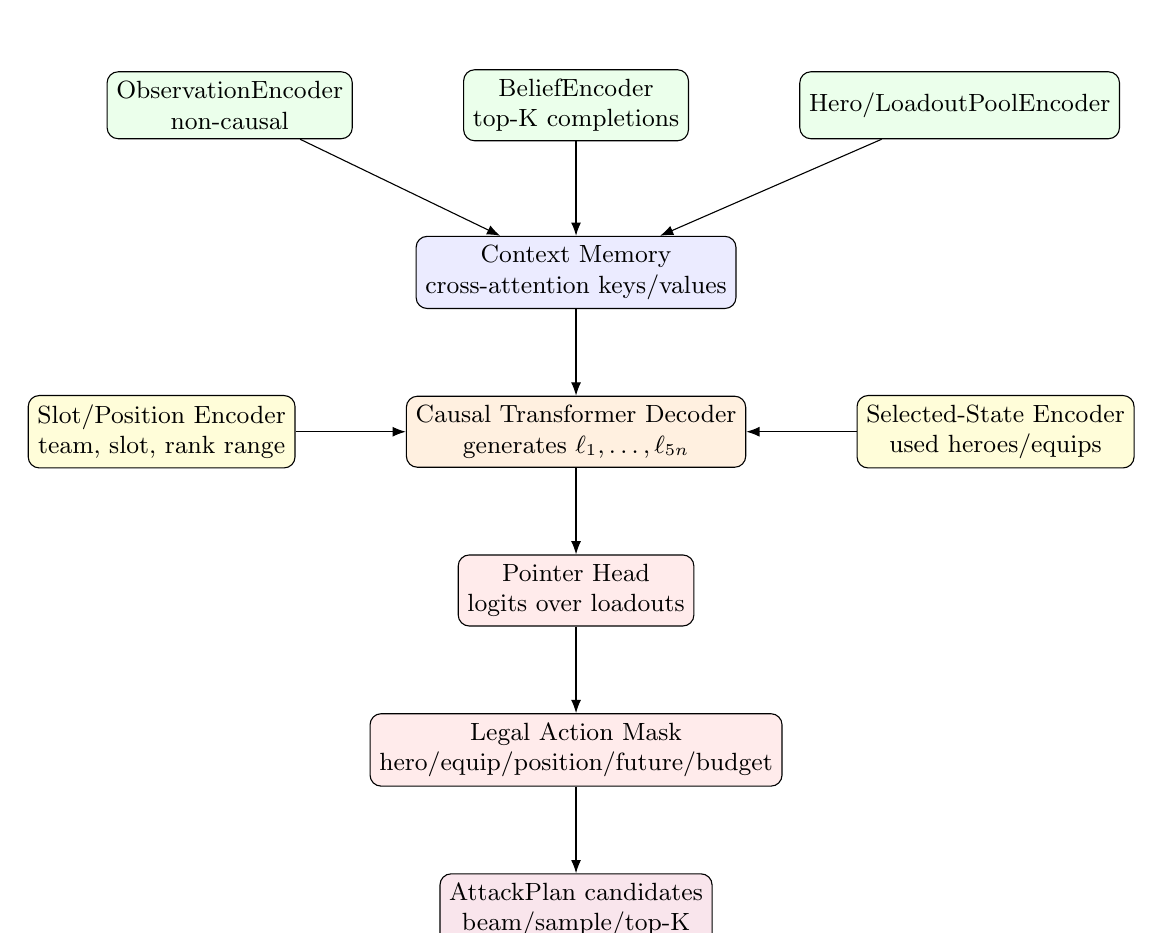
\begin{tikzpicture}[node distance=1.1cm and 1.4cm,>=Latex, every node/.style={font=\small}]
\tikzstyle{box}=[draw,rounded corners,align=center,minimum width=2.8cm,minimum height=0.85cm]
\node[box,fill=green!8] (obs) {ObservationEncoder\\non-causal};
\node[box,fill=green!8,right=of obs] (belief) {BeliefEncoder\\top-K completions};
\node[box,fill=green!8,right=of belief] (pool) {Hero/LoadoutPoolEncoder};
\node[box,fill=blue!8,below=1.2cm of belief] (context) {Context Memory\\cross-attention keys/values};
\node[box,fill=orange!12,below=of context] (dec) {Causal Transformer Decoder\\generates $\ell_1,\ldots,\ell_{5n}$};
\node[box,fill=yellow!15,left=of dec] (slot) {Slot/Position Encoder\\team, slot, rank range};
\node[box,fill=yellow!15,right=of dec] (state) {Selected-State Encoder\\used heroes/equips};
\node[box,fill=red!8,below=of dec] (ptr) {Pointer Head\\logits over loadouts};
\node[box,fill=red!8,below=of ptr] (mask) {Legal Action Mask\\hero/equip/position/future/budget};
\node[box,fill=purple!10,below=of mask] (out) {AttackPlan candidates\\beam/sample/top-K};
\draw[->] (obs) -- (context);
\draw[->] (belief) -- (context);
\draw[->] (pool) -- (context);
\draw[->] (context) -- (dec);
\draw[->] (slot) -- (dec);
\draw[->] (state) -- (dec);
\draw[->] (dec) -- (ptr);
\draw[->] (ptr) -- (mask);
\draw[->] (mask) -- (out);
\end{tikzpicture}}
\caption{AttackGenerationNetwork。感知端使用 non-causal encoder，生成端使用 causal decoder，合法性由 action mask 保证。}
\end{figure}

\section{ObservationEncoder}
每个 observation slot 编码为：
\begin{equation}
\begin{aligned}
x^O_{i,j}={}&Emb_{hero}(h_{i,j})+Emb_{equip}(u_{i,j})+Emb_{star}(s^u_{i,j})+Emb_{team}(i)\\
&+Emb_{slot}(j)+Emb_{hidden}(m_{i,j})+MLP([\rho,Power]).
\end{aligned}
\end{equation}
隐藏位置使用 learnable mask token。ObservationEncoder 使用 non-causal Transformer，因为所有可见信息在决策前已经可用。

\section{BeliefEncoder}
belief top-K 为 $\{(L^k,w_k)\}_{k=1}^{K}$。每个补全使用 PositionAwarePlanEncoder 得到 $z_{L^k}$，再加权聚合：
\begin{equation}
z_B=\sum_{k=1}^{K}w_k z_{L^k}.
\end{equation}
同时输入 belief entropy、top-1/top-2 差距和候选域大小等统计量。

\section{Causal Decoder}
当前生成序列为 $a_{<t}$。decoder 计算 query：
\begin{equation}
q_t=Dec^{causal}_\theta(a_{<t}, C_A, e_{slot_t}, e_{state_t}, e_{goal}).
\end{equation}
其中 $C_A$ 是由 observation、belief 和 loadout pool 编码组成的 context memory。

\section{Position-aware Candidate Scorer}
对候选 loadout $\ell$ 的分数为：
\begin{equation}
logit_t(\ell)=MLP([q_t,e_\ell,q_t\odot e_\ell,e_{slot_t},\phi_{pos}(\ell,s_t),\phi_{equip}(\ell),\phi_{underdog}(\ell)]).
\end{equation}
$\phi_{pos}$ 包括 standing rank、bucket、与上一槽位的 rank gap、未来可行性等。$\phi_{equip}$ 包括唯一装备 ID、星级、是否冲突、与 belief 防守的星级差。$\phi_{underdog}$ 包括当前 plan 成本、剩余预算、目标资源差。

\section{输出}
\begin{lstlisting}[caption={AttackNetOutput}]
@dataclass(frozen=True)
class AttackNetOutput:
    candidates: tuple[AttackPlan, ...]
    log_probs: tuple[float, ...]
    proposal_scores: tuple[float, ...]
    value_estimates: tuple[float, ...]
    legality_flags: tuple[bool, ...]
\end{lstlisting}

\section{训练}
训练样本来自 AttackOracle、真实平台成功进攻、Attack Exploiter 和 Underdog Attack Exploiter。基本损失：
\begin{equation}
\mathcal{L}_{attack}= -\sum_t\log P_\theta(a_t^*|O,g,a_{<t}^*)+\lambda_vMSE(\hat V,V^*)+\lambda_gMSE(\widehat{Gap},Gap^*).
\end{equation}

\section{下克上条件生成}
goal 参数包括 $target\_power\_ratio$。例如 0.9 表示希望进攻成本不超过防守 belief 平均成本的 90\%。decoder 的每一步 legal mask 应检查预算可行性：
\begin{equation}
C(A_{partial})+C(\ell)+MinFutureCost\le target\_power\_ratio\cdot \E_{L\sim b(L|O)}C(L).
\end{equation}
如果预算模式太严格导致无合法动作，应回退到软惩罚模式，而不是输出非法方案。


\chapter{DefenseRosterGenerationNetwork：防守 roster 生成网络}

\section{任务定义}
DefenseRosterGenerationNetwork 输入当前进攻 meta $\sigma_A$、防守方 loadout pool、目标条件和当前生成状态，输出合法 DefenseRoster 候选。它不直接选择 mask，mask 由 MaskSelectionNetwork 或 mask search 决定。

\section{攻击 meta 表示}
当前进攻 meta 是一组带权攻击方案：
\begin{equation}
\sigma_A=\{(A^1,w_1),\ldots,(A^K,w_K)\}.
\end{equation}
每个攻击方案使用 position-aware PlanEncoder 编码：
\begin{equation}
z_{A^k}=Enc_{plan}(A^k).
\end{equation}
meta 聚合：
\begin{equation}
z_{\sigma_A}=AttentionPool(\{z_{A^k}\},\{w_k\}).
\end{equation}

\section{网络结构}
防守网络结构为：AttackMetaEncoder、DefenseLoadoutPoolEncoder、Causal Roster Decoder、AntiMeta Candidate Scorer、Legal Action Mask、DefenseValueHead。

\begin{figure}[H]
\centering
\resizebox{0.96\textwidth}{!}{%
\begin{tikzpicture}[node distance=1.1cm and 1.4cm,>=Latex, every node/.style={font=\small}]
\tikzstyle{box}=[draw,rounded corners,align=center,minimum width=2.8cm,minimum height=0.85cm]
\node[box,fill=blue!8] (meta) {AttackMetaEncoder\\$\sigma_A$};
\node[box,fill=blue!8,right=of meta] (pool) {Defense Loadout Pool};
\node[box,fill=green!8,below=of meta] (ctx) {Defense Context\\anti-meta memory};
\node[box,fill=orange!12,below=of ctx] (dec) {Causal Roster Decoder\\generates $R$};
\node[box,fill=yellow!15,right=of dec] (legal) {Legal Action Mask\\hero/equip/position/future/budget};
\node[box,fill=purple!10,below=of dec] (roster) {DefenseRoster $R$};
\node[box,fill=green!8,below=of roster] (masknet) {MaskSelectionNetwork\\slot scorer + constrained selector};
\node[box,fill=red!8,below=of masknet] (defplan) {DefensePlan $D=(R,M)$};
\node[box,fill=gray!10,right=of masknet] (eval) {AttackOracle(O) 反打\\evaluate exploitability};
\draw[->] (meta) -- (ctx);
\draw[->] (pool) -- (ctx);
\draw[->] (ctx) -- (dec);
\draw[->] (legal) -- (dec);
\draw[->] (dec) -- (roster);
\draw[->] (roster) -- (masknet);
\draw[->] (masknet) -- (defplan);
\draw[->] (defplan) -- (eval);
\draw[->] (eval) .. controls +(-3.4,-0.8) and +(-2.5,0.3) .. (masknet.west);
\end{tikzpicture}}
\caption{Defense 网络。先生成合法 roster，再选择 mask，并用 AttackOracle 反打评估可被打穿程度。}
\end{figure}

\section{Roster 自回归生成}
\begin{equation}
P_\phi(R|\sigma_A,g_D)=\prod_{t=1}^{5n}P_\phi(r_t|\sigma_A,g_D,r_{<t}).
\end{equation}
decoder 使用 causal self-attention，cross-attend 到 attack meta context。

\section{AntiMeta Candidate Scorer}
候选 loadout $\ell$ 的防守生成分数：
\begin{equation}
\begin{aligned}
logit^D_t(\ell)=MLP([&q_t,e_\ell,e_{slot_t},q_t\odot e_\ell,
AntiMeta(\ell,\sigma_A),\\
&Maskability(\ell,s_t),PositionFeature(\ell,s_t),
UnderdogFeature(\ell)]).
\end{aligned}
\end{equation}

AntiMeta 表示该 loadout 对当前进攻 meta 的抑制价值，可以用 surrogate 近似边际收益：
\begin{equation}
AntiMeta(\ell,\sigma_A)\approx -\E_{A\sim\sigma_A}\Delta U(A,R_{partial}+\ell).
\end{equation}
Maskability 表示该 loadout 放在当前槽位后是否适合被隐藏。它和站位泄露、装备泄露、星级泄露以及 counter sensitivity 有关。

\section{合法性}
防守合法动作集合与攻击类似，但使用防守方 loadout pool。必须满足：英雄未使用、唯一装备 ID 未使用、站位顺序合法、未来可补齐、资源预算可行。

\section{训练}
训练样本来自 DefenseOracle、真实平台高表现防守、Defense Exploiter 和 Underdog Defense Exploiter。损失：
\begin{equation}
\begin{aligned}
\mathcal{L}_{def}={}&-\sum_t\log P_\phi(r_t^*|\sigma_A,g_D,r_{<t}^*)\\
&+\lambda_vMSE(\hat V_D,V_D^*)+\lambda_mMSE(\widehat{Maskability},Maskability^*).
\end{aligned}
\end{equation}

\section{防守下克上}
防守侧 goal 参数表示希望用低资源防守抵抗更高资源攻击。目标可写为：
\begin{equation}
\begin{aligned}
J_D(R,M)=&-\E_{A\sim\sigma_A}U(A,R)
+\lambda_u\E_{A\sim\sigma_A}\max(0,Gap_D(A,R))\\
&+\lambda_M \mathrm{Ambiguity}(\Observe(R,M))-\lambda_C C(R).
\end{aligned}
\end{equation}
这使防守生成网络不只学习堆高资源，而会学习低资源抗强攻的结构。


\chapter{MaskSelectionNetwork：隐藏位置选择网络}

\section{任务定义}
MaskSelectionNetwork 输入完整防守 roster $R$ 和当前攻击 meta $\sigma_A$，输出合法 mask $M$。它的目标不是简单隐藏强英雄，而是让攻击方看到 observation 后存在多个可行补全，并且这些补全需要不同 counter。

\section{为什么不推荐独立二分类}
如果对每个槽位独立预测 hide/visible，容易违反每队最多隐藏 2 个、全局最多隐藏 10 个的约束，也无法考虑隐藏组合之间的相互作用。推荐使用 SlotScorer + ConstrainedSelector。

\section{SlotScorer}
对每个槽位 $(i,j)$，计算隐藏价值：
\begin{equation}
\begin{aligned}
q_{i,j}=MLP([&z_{R,i,j},z_{\sigma_A},CoreValue_{i,j},PositionLeakage_{i,j},\\
&EquipLeakage_{i,j},StarUncertainty_{i,j},CounterSensitivity_{i,j}]).
\end{aligned}
\end{equation}

各项含义如下：
\begin{longtable}{p{0.25\linewidth}p{0.68\linewidth}}
\toprule
特征 & 含义 \\
\midrule
CoreValue & 该位置是否承载阵容核心或胜负手。\\
PositionLeakage & 隐藏后是否仍能被站位边界轻易推断。候选域越小，泄露越高。\\
EquipLeakage & 可见唯一装备是否已暴露体系，导致隐藏位容易被推出。\\
StarUncertainty & 3-5 星差异是否影响攻击方 counter 选择。\\
CounterSensitivity & 隐藏该位置后，AttackOracle 输出是否发生显著变化。\\
\bottomrule
\end{longtable}

\section{组合选择目标}
mask 选择可写为约束优化：
\begin{equation}
M^*=\arg\max_M\sum_{i,j}q_{i,j}M_{i,j}+\lambda_HH(b(L|O))+\lambda_C\log(|\Ccal_L(O)|+1)-\lambda_AAttackSuccess(O,R).
\end{equation}
其中 $O=\Observe(R,M)$。
约束：
\begin{align}
\sum_jM_{i,j}&\le 2,\\
\sum_{i,j}M_{i,j}&\le 10.
\end{align}

\section{BO3 与 BO5 的 mask 搜索}
每队最多隐藏 0、1、2 个，因此每队 pattern 数为
\begin{equation}
\binom{5}{0}+\binom{5}{1}+\binom{5}{2}=16.
\end{equation}
BO3 全量 mask 数量为 $16^3=4096$，可以枚举。BO5 为 $16^5=1,048,576$，不建议每个都调用 AttackOracle，应使用 beam search。

\begin{lstlisting}[caption={BO5 mask beam search}]
def beam_search_masks(roster, beam_size):
    beam = [empty_mask_state()]
    for team_idx in range(format.n_teams):
        new_beam = []
        for state in beam:
            for pattern in legal_team_mask_patterns():
                candidate = state.add_pattern(team_idx, pattern)
                approx_score = mask_scorer.approx(candidate, roster)
                new_beam.append((candidate, approx_score))
        beam = top_k_with_diversity(new_beam, beam_size)
    return beam
\end{lstlisting}

\section{训练}
训练样本来自对固定 roster 枚举/搜索得到的最佳 mask。可以使用 ranking loss：
\begin{equation}
\mathcal{L}_{mask}=-\log\frac{\exp(score(M^*)/\tau)}{\sum_{M'\in\mathcal{M}(R)}\exp(score(M')/\tau)}.
\end{equation}


\chapter{BeliefModel：从隐藏观测到 loadout belief}

\section{任务定义}
BeliefModel 输入 observation $O$，输出在可行补全集合上的概率分布 $b(L|O)$。这里 $L$ 是完整 loadout roster，包含隐藏英雄、唯一装备 ID、唯一装备星级、普通装备、练度、战力和站位。

\section{V1：检索式 belief}
第一版推荐使用检索式 belief。从 DefensePool 和 RealMetaDB 中找到与 $O$ 兼容的防守，先经过 ConstraintEngine 检查，再用频率和强度加权。
\begin{equation}
w(L|O)\propto freq_{real}(L|O)^\alpha strength(L)^\beta recency(L)^\gamma sim(L,O)^\eta.
\end{equation}
归一化：
\begin{equation}
b(L|O)=\frac{w(L|O)}{\sum_{L'}w(L'|O)}.
\end{equation}

\section{V2：候选 ranking belief}
如果可行补全数量较多，先从 $\Ccal_L(O)$ 中采样或 beam 得到 top-K，然后训练候选打分网络。
Observation encoder：
\begin{equation}
z_O=Enc_O(O).
\end{equation}
Candidate roster encoder：
\begin{equation}
z_L=Enc_L(L).
\end{equation}
兼容分数：
\begin{equation}
q_\theta(L,O)=MLP([z_O,z_L,z_O\odot z_L,z_O-z_L,features(L,O)]).
\end{equation}
概率：
\begin{equation}
b_\theta(L|O)=\frac{1[L\in\Ccal_L(O)]\exp(q_\theta(L,O)/\tau)}{\sum_{L'\in\Ccal_L(O)}\exp(q_\theta(L',O)/\tau)}.
\end{equation}

\section{V3：自回归补全}
如果需要生成未知补全，可以使用 causal decoder：
\begin{equation}
P(L_{hidden}|O)=\prod_{t=1}^{Z}P(\ell_t|O,\ell_{<t}).
\end{equation}
每一步的 action mask 是当前隐藏槽位的 $\Omega_s(O)$，并额外删除已补过的英雄和唯一装备 ID。

\section{训练数据}
训练数据来自真实平台。每条样本为 $(O,L^+)$，其中 $L^+$ 是赛后可见或回放得到的完整防守 loadout。如果无法得到完整装备星级，可将星级作为 latent variable，用边缘似然或 EM 风格估计。

\section{输出契约}
BeliefEngine 输出必须包含：
\begin{lstlisting}[caption={BeliefOutput}]
@dataclass(frozen=True)
class BeliefOutput:
    candidates: tuple[DefenseRoster, ...]
    weights: tuple[float, ...]
    entropy: float
    feasible_count_estimate: int
    top1_top2_gap: float
    domain_stats: dict[str, float]
\end{lstlisting}

AttackOracle 必须只在 BeliefOutput.candidates 上求期望，不允许在未经过合法性检查的补全上打分。


\chapter{AttackOracle：完整搜索流程}

\section{职责}
AttackOracle 的职责是给定完整防守 $L$ 或 observation $O$，输出经过仿真复评的 top-K 合法进攻方案。它不是神经网络，而是组合搜索系统。

\section{完整信息版本}
完整信息目标：
\begin{equation}
A^*(L)=\arg\max_{A:\LegalAttack_n(A)=1}J_A(A,L).
\end{equation}
其中 $J_A$ 可以是普通胜率，也可以是下克上目标。

流程：生成合法 N 队进攻候选，使用 SingleTeamWinrateModel 估计每路胜率，使用 DP 计算整体胜率，做多样性筛选，使用 Successive Halving 仿真复评，输出最终方案。

\section{mask observation 版本}
mask 信息目标：
\begin{equation}
A^*(O)=\arg\max_{A:\LegalAttack_n(A)=1}\sum_{k=1}^{K}b(L^k|O)J_A(A,L^k).
\end{equation}

\section{候选生成混合策略}
候选来源应混合：
\begin{longtable}{p{0.30\linewidth}p{0.62\linewidth}}
\toprule
来源 & 目的 \\
\midrule
合法随机完整 N 队 & 保持全局探索。\\
AttackGenerationNetwork & 生成高质量 proposal。\\
Mutation from top attacks & 局部优化已知强方案。\\
Crossover & 组合两个强方案的不同队伍结构。\\
LCB candidates & 稳健可用。\\
UCB candidates & 探索模型不确定但可能强的区域。\\
Low-resource candidates & 支持下克上。\\
Long-tail coverage & 防止冷门英雄永远没机会。\\
\bottomrule
\end{longtable}

\section{多样性选择}
多样性得分：
\begin{equation}
Score(A)=Value(A)+\alpha Div(A)-\beta ResourceOverlap(A)-\gamma SimilarityToSelected(A).
\end{equation}
其中 Similarity 可以用英雄集合 Jaccard：
\begin{equation}
sim(A,B)=\frac{|Heroes(A)\cap Heroes(B)|}{|Heroes(A)\cup Heroes(B)|}.
\end{equation}

\section{Successive Halving}
\begin{lstlisting}[caption={AttackOracle 多保真流程}]
def attack_oracle(input, budget):
    belief = build_belief_if_needed(input)
    candidates = generate_legal_attack_candidates(input, N=100000)
    scored = surrogate_score(candidates, belief)
    pool = diversity_select(scored, K=5000)

    pool = simulate_and_keep(pool, games_each=3, keep=1000)
    pool = simulate_and_keep(pool, games_each=10, keep=200)
    pool = simulate_and_keep(pool, games_each=50, keep=20)
    pool = simulate_and_keep(pool, games_each=200, keep=5)
    return rank_by_calibrated_real_value(pool)
\end{lstlisting}

\section{风险报告}
AttackOracle 输出不应只有一个方案，还应输出风险解释：belief top candidates、每路预测胜率、uncertainty、关键假设、如果隐藏星级为 5 星时的 worst-case 胜率、备用方案。


\chapter{DefenseOracle：防守 roster 与 mask 的联合决策}

\section{职责}
DefenseOracle 的职责是输出一个 DefensePlan $D=(R,M)$，使当前 AttackOracle 看到 $O=\Observe(R,M)$ 后仍然难以打穿。它必须同时考虑阵容真实强度、mask 迷惑性、真实平台进攻分布和下克上目标。

\section{目标函数}
\begin{equation}
D^*=\arg\max_{R,M}\; J_D(R,M).
\end{equation}
其中
\begin{equation}
\begin{aligned}
J_D(R,M)=&-\mathrm{AttackSuccess}(R,M)+\lambda_H H(b(L|O))\\
&+\lambda_C\log(|\Ccal_L(O)|+1)
+\lambda_U \mathrm{UnderdogDefense}(R)-\lambda_R C(R).
\end{aligned}
\end{equation}

\section{两阶段生成}
第一阶段生成 roster $R$。第二阶段选择 mask $M$。这种分解更容易保证合法性，也更容易调试。

\section{防守候选生成}
候选来源包括：合法随机、DefenseRosterGenerationNetwork、从强防守 mutation、从两个防守 crossover、针对当前强进攻的 Defense Exploiter、低资源 Underdog Defense Exploiter。

\section{mask 选择与反打评估}
每个 roster 先得到若干 mask 候选。对每个 $(R,M)$：
\begin{enumerate}[leftmargin=2em]
\item 计算 $O=\Observe(R,M)$。
\item BeliefEngine 构造 $b(L|O)$。
\item AttackOracle 输出 $A^*(O)$。
\item 在真实 $R$ 上评估 $U(A^*(O),R)$。
\item 记录 attack success、ambiguity、leakage 和 underdog defense gap。
\end{enumerate}

\section{防守输出}
防守输出应包含：主方案、备用方案、预估被打穿率、mask 解释、最可能被哪类进攻打穿、建议的历史池标签。

\begin{lstlisting}[caption={DefenseOracle 输出结构}]
@dataclass(frozen=True)
class DefenseOracleOutput:
    best_defense: DefensePlan
    backup_defenses: tuple[DefensePlan, ...]
    estimated_attack_success: float
    ambiguity_score: float
    worst_case_attack: AttackPlan
    explanation: dict[str, str]
\end{lstlisting}


\chapter{ActivePerceptionScheduler：主动感知与未知区域探索}

\section{为什么需要主动感知}
只靠随机仿真会浪费大量预算；只靠当前强阵容附近搜索会导致策略塌缩。主动感知模块负责选择下一批最有信息价值的仿真或真实采集任务。

\section{Query 类型}
查询 $q$ 可以是：单队 matchup、完整 match、mask observation、防守 mask 组合、星级不确定区域、站位边界样本、低资源反制样本、top1/top2 决策边界样本。

\section{Acquisition 函数}
\begin{equation}
\begin{aligned}
Acq(q)=&\lambda_1InfoGain(q)+\lambda_2DecisionImpact(q)+\lambda_3MetaFreq(q)\\
&+\lambda_4Novelty(q)+\lambda_5UnderdogPotential(q)-\lambda_6Cost(q).
\end{aligned}
\end{equation}

\section{InfoGain}
可以用 ensemble disagreement、predictive entropy 或 belief entropy 近似。对单队 matchup：
\begin{equation}
InfoGain(A_i,L_i)\approx Var_k[f_k(A_i,L_i)].
\end{equation}
对 observation：
\begin{equation}
InfoGain(O)\approx H(b(L|O)).
\end{equation}

\section{DecisionImpact}
如果当前 top-1 和 top-2 进攻分数接近，该 observation 采样价值高。定义
\begin{equation}
DecisionImpact(O)=\exp\left(-\frac{Score(A_1|O)-Score(A_2|O)}{\tau}\right).
\end{equation}

\section{UnderdogPotential}
\begin{equation}
UnderdogPotential(A,L)=1[C(A)<C(L)]\cdot UCB(CounterResidual(A,L)).
\end{equation}
它鼓励系统主动仿真低资源可能反制高资源的组合。

\begin{figure}[H]
\centering
\resizebox{0.92\textwidth}{!}{%
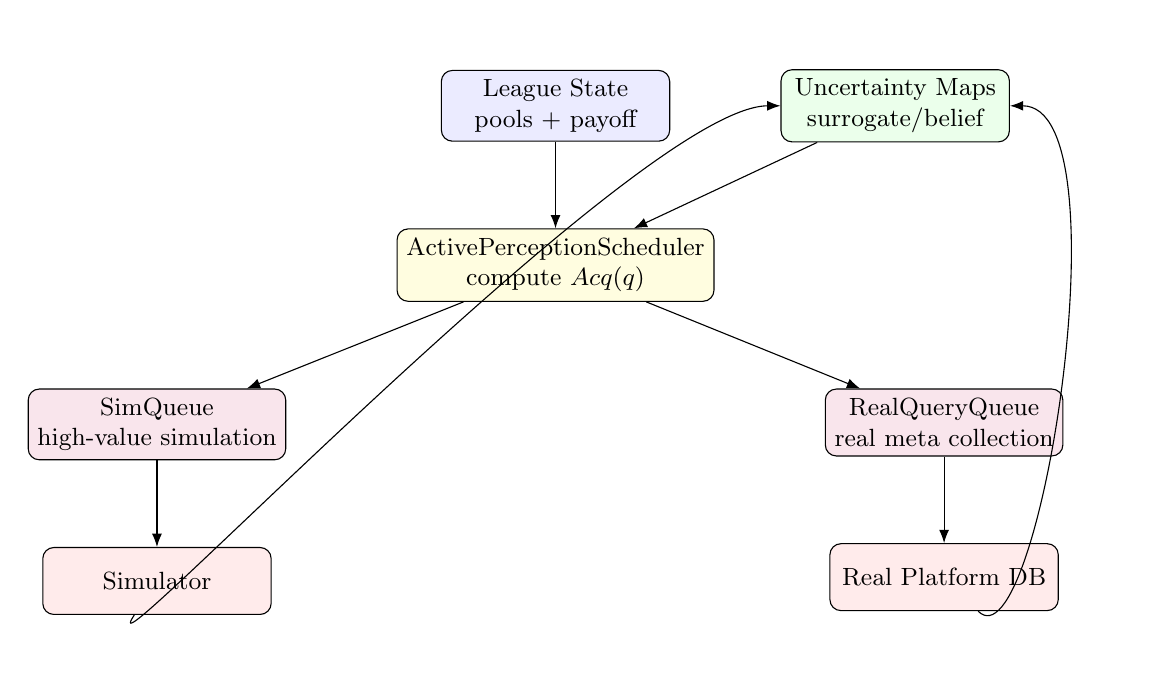
\begin{tikzpicture}[node distance=1.1cm and 1.4cm,>=Latex, every node/.style={font=\small}]
\tikzstyle{box}=[draw,rounded corners,align=center,minimum width=2.9cm,minimum height=0.85cm]
\node[box,fill=blue!8] (league) {League State\\pools + payoff};
\node[box,fill=green!8,right=of league] (unc) {Uncertainty Maps\\surrogate/belief};
\node[box,fill=yellow!12,below=of league] (sched) {ActivePerceptionScheduler\\compute $Acq(q)$};
\node[box,fill=purple!10,below left=of sched] (simq) {SimQueue\\high-value simulation};
\node[box,fill=purple!10,below right=of sched] (realq) {RealQueryQueue\\real meta collection};
\node[box,fill=red!8,below=of simq] (sim) {Simulator};
\node[box,fill=red!8,below=of realq] (real) {Real Platform DB};
\draw[->] (league) -- (sched);
\draw[->] (unc) -- (sched);
\draw[->] (sched) -- (simq);
\draw[->] (sched) -- (realq);
\draw[->] (simq) -- (sim);
\draw[->] (realq) -- (real);
\draw[->] (sim) .. controls +(-1.0,-1.5) and +(-1.8,0) .. (unc.west);
\draw[->] (real) .. controls +(1.2,-1.2) and +(1.5,0) .. (unc.east);
\end{tikzpicture}}
\caption{主动感知调度。系统不随机探索，而是根据信息增益、决策影响、真实 meta 频率、新颖性、下克上潜力和成本选择下一批任务。}
\end{figure}

\section{输出队列}
ActivePerceptionScheduler 输出两个队列：SimQueue 和 RealQueryQueue。SimQueue 发给仿真器，RealQueryQueue 用于真实平台重点记录和重点测试。


\chapter{RealCalibrationModel 与真实平台数据闭环}

\section{问题}
仿真胜率 $P_{sim}$ 与真实平台胜率 $P_{real}$ 不一致。真实平台有真实玩家偏好、装备星级分布、mask 习惯、分段差异和赛季变化。系统最终优化的应该是 $P_{real}$。

\section{RealMetaDB 字段}
\begin{longtable}{p{0.28\linewidth}p{0.62\linewidth}}
\toprule
字段 & 含义 \\
\midrule
observation\_hash & mask observation 的规范化哈希。\\
visible\_slots & 可见槽位，包括英雄、装备、星级、战力摘要。\\
hidden\_slots & 隐藏位置列表。\\
full\_defense\_if\_available & 赛后可回看时记录完整防守。\\
attack\_plan & 实际进攻方案。\\
lane\_results & 每路胜负、时长、剩余血量。\\
match\_result & BO3/BO5 整体结果。\\
unique\_equip\_stars & 唯一传奇装备星级。\\
rank\_segment & 真实平台分段。\\
server & 服务器或环境。\\
season & 赛季/版本。\\
timestamp & 时间戳。\\
\bottomrule
\end{longtable}

\section{校准模型}
简单校准：
\begin{equation}
\logit(p_{real})=a\cdot\logit(p_{sim})+b+\gamma^\top x.
\end{equation}
其中 $x$ 包含赛季、分段、装备星级、真实频率等。也可以使用小 MLP：
\begin{equation}
p_{real}=Calibrator(p_{sim},x).
\end{equation}

\section{真实分布 belief}
mask 下攻击目标应使用：
\begin{equation}
A^*(O)=\arg\max_A\E_{L\sim P_{real}(L|O)}[U_{real}(A,L)].
\end{equation}
真实数据库负责估计 $P_{real}(L|O)$，仿真负责探索未知策略空间。

\section{版本漂移}
每个模型和数据都必须带版本字段。赛季切换后，RealCalibrationModel 和 BeliefModel 应提高近期数据权重，降低旧数据权重。建议使用指数衰减：
\begin{equation}
w_{time}=\exp(-\Delta t/\tau_{season}).
\end{equation}


\chapter{LeagueManager：AlphaStar-style PSRO}

\section{策略池}
维护攻击池和防守池：
\begin{equation}
\Pi_A=\{A^1,\ldots,A^m\},\quad \Pi_D=\{D^1,\ldots,D^k\}.
\end{equation}
防守策略 $D^j=(R^j,M^j)$。

\section{Payoff Matrix}
\begin{equation}
P_{ij}=U(A^i,R^j).
\end{equation}
攻击收益 $u_A=P_{ij}$，防守收益 $u_D=1-P_{ij}$。

\section{Meta 分布}
第一版使用混合采样：
\begin{equation}
\sigma=0.4\sigma_{strong}+0.3\sigma_{historical}+0.2\sigma_{diverse}+0.1\sigma_{random}.
\end{equation}
后续可替换为 Nash、replicator dynamics 或 AlphaRank。

\section{策略角色}
Main Attack：
\begin{equation}
A_{main}=\arg\max_A\E_{D\sim\sigma_D}U(A,D).
\end{equation}
Attack Exploiter：
\begin{equation}
A_{exp}=BR(D_{hard}).
\end{equation}
Main Defense：
\begin{equation}
D_{main}=\arg\min_D\E_{A\sim\sigma_A}U(A,D).
\end{equation}
Defense Exploiter：
\begin{equation}
D_{exp}=BR(A_{strong}).
\end{equation}
Underdog Exploiter：专门搜索低资源反制高资源策略。

\begin{figure}[H]
\centering
\resizebox{0.93\textwidth}{!}{%
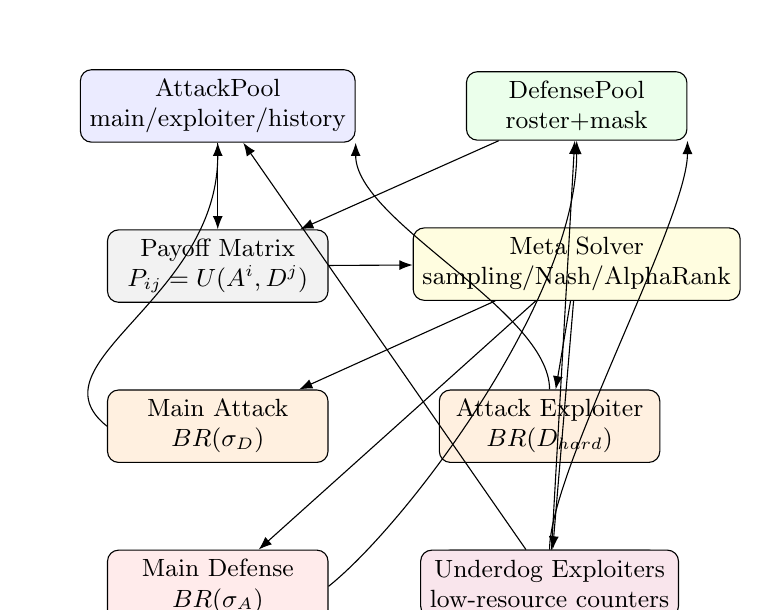
\begin{tikzpicture}[node distance=1.1cm and 1.4cm,>=Latex, every node/.style={font=\small}]
\tikzstyle{box}=[draw,rounded corners,align=center,minimum width=2.8cm,minimum height=0.85cm]
\node[box,fill=blue!8] (apool) {AttackPool\\main/exploiter/history};
\node[box,fill=green!8,right=of apool] (dpool) {DefensePool\\roster+mask};
\node[box,fill=gray!10,below=of apool] (matrix) {Payoff Matrix\\$P_{ij}=U(A^i,D^j)$};
\node[box,fill=yellow!12,below=of dpool] (meta) {Meta Solver\\sampling/Nash/AlphaRank};
\node[box,fill=orange!12,below=of matrix] (mainA) {Main Attack\\$BR(\sigma_D)$};
\node[box,fill=orange!12,right=of mainA] (expA) {Attack Exploiter\\$BR(D_{hard})$};
\node[box,fill=red!8,below=of mainA] (mainD) {Main Defense\\$BR(\sigma_A)$};
\node[box,fill=red!8,right=of mainD] (expD) {Defense Exploiter\\$BR(A_{strong})$};
\node[box,fill=purple!10,below=of expA] (under) {Underdog Exploiters\\low-resource counters};
\draw[->] (apool) -- (matrix);
\draw[->] (dpool) -- (matrix);
\draw[->] (matrix) -- (meta);
\draw[->] (meta) -- (mainA);
\draw[->] (meta) -- (expA);
\draw[->] (meta) -- (mainD);
\draw[->] (meta) -- (expD);
\draw[->] (mainA.west) .. controls +(-1.0,0.8) and +(0,-2.0) .. (apool.south);
\draw[->] (expA.north) .. controls +(0,1.0) and +(0,-1.0) .. (apool.south east);
\draw[->] (mainD.east) .. controls +(1.0,0.8) and +(0,-2.0) .. (dpool.south);
\draw[->] (expD.north) .. controls +(0,1.0) and +(0,-1.0) .. (dpool.south east);
\draw[->] (under) -- (apool);
\draw[->] (under) -- (dpool);
\end{tikzpicture}}
\caption{AlphaStar-style League + PSRO。main 策略追求泛化，exploiter 找漏洞，underdog exploiter 专门寻找低资源反制。}
\end{figure}

\section{League Iteration}
\begin{lstlisting}[caption={League 训练循环}]
while True:
    update_payoff_matrix(AttackPool, DefensePool)
    sigma_A, sigma_D = compute_meta_distributions()

    A_main = AttackOracle(defense_meta=sigma_D, role="main")
    A_exp  = AttackOracle(target=hardest_defense(), role="exploiter")
    A_under = AttackOracle(target=hardest_defense(), role="underdog")
    AttackPool.add(A_main, A_exp, A_under)

    D_main = DefenseOracle(attack_meta=sigma_A, role="main")
    D_exp  = DefenseOracle(target=strongest_attack(), role="exploiter")
    D_under = DefenseOracle(target=strongest_attack(), role="underdog")
    DefensePool.add(D_main, D_exp, D_under)

    ActivePerceptionScheduler.schedule_next_queries()
    RealCalibrationModel.update_if_real_data_available()
\end{lstlisting}

\section{保留历史策略}
不要只保留最新策略。历史策略防止遗忘，尤其用于防止系统只适应当前一轮 exploiters。弱策略可以降权，但不应立即删除；如果一个旧策略在新 meta 下重新变强，应允许重新升权。


\chapter{数据工程规范：表结构、缓存、哈希与可复现性}

\section{规范化哈希}
所有 Team、AttackPlan、DefensePlan、Observation 都必须有 canonical hash。队内顺序由站位固定，队伍顺序如果固定对位则不可交换；如果游戏允许重排，则 hash 前应先 canonicalize。

\section{核心表}
\subsection{LoadoutTable}
记录每个 loadout 的英雄、装备、星级、普通装备、属性、站位、战力和版本。
\subsection{SingleMatchupTable}
记录单队 matchup 的仿真/真实结果。
\subsection{PlanMatchTable}
记录完整 BO3/BO5 plan 对战结果。
\subsection{ObservationTable}
记录 mask observation、兼容补全、真实频率和 belief 统计。
\subsection{LeagueStrategyTable}
记录 AttackPool 和 DefensePool 里的策略来源、角色、创建时间、表现和多样性 cluster。

\section{缓存键}
单队 matchup cache key 应包含：attack team hash、defense team hash、版本、装备星级、仿真器版本、随机种子策略。完整 match cache key 应包含 AttackPlan hash、DefensePlan roster hash、format、版本。

\section{可复现性}
每次输出都应记录：模型版本、数据版本、仿真器版本、league iteration、随机种子、候选生成配置、校准模型版本。

\begin{lstlisting}[caption={ResultMetadata}]
@dataclass(frozen=True)
class ResultMetadata:
    model_version: str
    data_version: str
    simulator_version: str
    league_iteration: int
    random_seed: int
    generation_config_hash: str
    calibration_version: str
\end{lstlisting}


\chapter{训练流程：从仿真预训练到真实平台校准}

\section{阶段 1：仿真覆盖数据}
先生成大量合法单队和完整 N 队样本，覆盖英雄、站位、唯一装备星级和普通装备配置。采样不能只来自强阵容，否则模型会只在强阵容附近准确。

\section{阶段 2：SingleTeamWinrateModel}
训练 position-aware、star-aware 的单队胜率模型。数据包含随机样本、边界样本、高不确定样本、下克上样本和真实校准样本。

\section{阶段 3：AttackOracle 产生老师}
使用合法生成、surrogate 和仿真复评产生强进攻。输出样本用于训练 AttackGenerationNetwork。

\section{阶段 4：DefenseOracle 产生老师}
生成防守 roster 和 mask，用 AttackOracle 反打，筛出难打防守。输出样本用于训练 DefenseRosterGenerationNetwork 和 MaskSelectionNetwork。

\section{阶段 5：League 自博弈}
进入 AttackPool/DefensePool 循环，不断产生 main、exploiter、underdog 策略。

\section{阶段 6：真实平台校准}
真实平台数据回流后，训练 RealCalibrationModel 和真实频率 belief。采样权重逐渐从仿真探索转向真实 meta。

\section{训练配比建议}
前期：70\% 仿真覆盖，20\% 主动不确定，10\% 人工/真实。中期：50\% 仿真，30\% league，20\% 真实。后期：40\% 仿真探索，30\% league，30\% 真实校准。


\chapter{评估指标与实验协议}

\section{单队模型指标}
Accuracy 只能作为粗指标。更重要的是 AUC、Brier、ECE、Precision@K、Recall@K、高分候选真实复评胜率、下克上样本召回率。

\section{AttackOracle 指标}
\begin{longtable}{p{0.30\linewidth}p{0.62\linewidth}}
\toprule
指标 & 说明 \\
\midrule
Top-1 real winrate & 最终推荐进攻真实/仿真胜率。\\
Top-5 hit rate & 前 5 个方案中是否有可用方案。\\
Belief robustness & 对 belief top-K 防守的平均胜率和 worst-case 胜率。\\
Resource efficiency & 胜率除以资源成本，或约束资源下胜率。\\
Underdog success & 低资源打高资源成功率。\\
\bottomrule
\end{longtable}

\section{DefenseOracle 指标}
关注 attack success rate、mask ambiguity、belief entropy、被 best response 打穿率、真实平台防守成功率、低资源防守成功率。

\section{League 指标}
关注策略池多样性、exploitability 近似、payoff matrix 非传递性、历史策略复活率、meta 稳定性和真实平台胜率。

\section{Ablation}
必须做以下消融：去掉站位特征、去掉装备星级、去掉 action mask 的 future feasibility、去掉 underdog objective、去掉 mask ambiguity、去掉真实校准、去掉 active perception。


\chapter{工程落地路线与任务拆分}

\section{Phase 1：数据结构和合法性}
实现 MatchFormat、HeroRecord、Loadout、Team、AttackPlan、DefensePlan、Observation、ConstraintEngine。所有生成器必须先通过 legality tests。

\section{Phase 2：完整防守版 AttackOracle}
不处理 mask，输入完整 roster，输出进攻方案。这是第一个 MVP。

\section{Phase 3：仿真缓存与 Hyperband}
所有仿真结果写缓存。实现分层预算评估。不要对所有候选平均分配预算。

\section{Phase 4：BeliefEngine}
实现 BuildDomains、MRV、forward checking、completion ranking。把 belief 从 hero 扩展到 loadout，包括装备星级。

\section{Phase 5：mask-aware AttackOracle}
输入 observation，输出对 belief 加权最优的进攻。

\section{Phase 6：DefenseOracle}
先生成 roster，再搜索 mask，并用 AttackOracle 反打。

\section{Phase 7：生成网络蒸馏}
用 Oracle 输出训练 AttackGenerationNetwork、DefenseRosterGenerationNetwork、MaskSelectionNetwork。

\section{Phase 8：LeagueManager}
建立 AttackPool、DefensePool、payoff matrix、main/exploiter/underdog 角色。

\section{Phase 9：真实平台闭环}
实现 RealMetaDB、RealCalibrationModel、ActivePerceptionScheduler 和真实分布重加权。


\chapter{测试、验收标准与失败模式}

\section{合法性单元测试}
必须覆盖：英雄重复、唯一装备重复、站位顺序错误、mask 超过每队上限、mask 超过全局上限、隐藏补全不匹配可见槽、装备星级字段缺失。

\section{网络输出测试}
攻击和防守生成网络输出必须 100\% 合法。任何非法输出都表示 action mask 或 forward feasibility 有 bug，而不是模型质量问题。

\section{Belief 测试}
给定人工构造 observation，应能排除站位不可能英雄、已出现英雄、已使用唯一装备。真实完整防守必须属于 $\Ccal_L(O)$。如果不属于，说明观测或规则实现有问题。

\section{下克上测试}
构造固定高资源防守，检查系统是否能搜索低资源候选，并报告 underdog gap。若所有 top 方案都是最高资源堆叠，说明 underdog objective、采样或 residual model 未生效。

\section{常见失败模式}
\begin{longtable}{p{0.30\linewidth}p{0.62\linewidth}}
\toprule
失败模式 & 排查方向 \\
\midrule
候选高度同质 & 多样性选择、hero histogram、低资源分桶是否生效。\\
高分候选仿真翻车 & 校准、uncertainty、LCB 权重、数据泄漏。\\
mask 隐藏无效 & PositionLeakage 和 EquipLeakage 没有进入 mask scorer。\\
真实平台效果差 & RealCalibrationModel、真实频率 belief、版本漂移。\\
下克上失败 & counter residual、underdog sampling、资源成本定义。\\
\bottomrule
\end{longtable}


\chapter{给执行模型的标准作业流程}

\section{实现模型应遵循的顺序}
执行模型不得从训练大模型开始。正确顺序是：先实现数据结构和合法性，再实现完整防守 AttackOracle，再实现仿真缓存，再加入 belief，再加入防守，再加入生成网络蒸馏，最后接 league 和真实平台。

\section{每个模块的输入输出必须固定}
每个模块必须使用本文定义的数据结构，不允许临时使用 list of ids 代替 loadout。尤其 unique equip star、standing rank、final power 必须贯穿数据管线。

\section{每次输出必须包含解释}
进攻输出必须包含 belief top-K、防守补全权重、每路胜率、总胜率、风险、备用方案和下克上 gap。防守输出必须包含 mask 理由、可行补全集合大小、belief entropy、最强反打方案和被打穿风险。

\section{执行模型的禁止事项}
\begin{enumerate}[leftmargin=2em]
\item 不允许让网络自由输出后再过滤作为主流程。
\item 不允许在没有仿真复评时直接使用生成网络 top-1。
\item 不允许忽略站位顺序。
\item 不允许把唯一装备星级当成唯一性 key。
\item 不允许只在仿真随机分布上做最终决策。
\item 不允许只优化胜率而完全不记录资源成本。
\end{enumerate}

\section{最小可交付版本}
最小可交付版本必须包含：MatchFormat、Loadout、合法生成器、SingleTeamWinrateModel 接口、完整防守 AttackOracle、仿真缓存、Successive Halving、多样性选择、输出解释。


\chapter{配置模板与接口契约}

\section{YAML 配置示例}
\begin{lstlisting}[caption={系统配置示例}]
match_format:
  n_teams: 5
  team_size: 5
  win_required: 3
  max_hidden_per_team: 2
  max_hidden_total: 10

surrogate:
  ensemble_size: 5
  lcb_beta: 1.0
  ucb_beta: 1.0
  calibration: temperature

candidate_generation:
  num_random: 50000
  num_policy: 30000
  num_mutation: 15000
  num_underdog: 5000
  diversity_threshold: 0.7

underdog:
  enabled: true
  target_power_ratios: [1.0, 0.9, 0.8]
  residual_weight: 0.5

hyperband:
  stages:
    - games_each: 3
      keep: 1000
    - games_each: 10
      keep: 200
    - games_each: 50
      keep: 20
    - games_each: 300
      keep: 5
\end{lstlisting}

\section{模块接口总表}
\begin{longtable}{p{0.28\linewidth}p{0.30\linewidth}p{0.32\linewidth}}
\toprule
模块 & 输入 & 输出 \\
\midrule
ConstraintEngine & Observation / Plan & domains, completions, legality flag \\
BeliefEngine & Observation & BeliefOutput \\
SurrogateScorer & Team vs Team & $\mu,\sigma,margin,time,residual$ \\
AttackGenerationNetwork & Observation, belief, pool, goal & Attack candidates \\
DefenseRosterGenerationNetwork & attack meta, pool, goal & roster candidates \\
MaskSelectionNetwork & roster, attack meta & mask candidates \\
AttackOracle & roster or observation & ranked AttackPlan \\
DefenseOracle & attack meta & ranked DefensePlan \\
ActivePerceptionScheduler & league state, uncertainty & SimQueue, RealQueryQueue \\
RealCalibrationModel & sim score, context & calibrated real score \\
\bottomrule
\end{longtable}


\chapter{附录 A：关键伪代码}

\section{match win probability}
\begin{lstlisting}[caption={BO3/BO5 通用胜率 DP}]
def match_win_prob(ps: list[float], win_required: int) -> float:
    n = len(ps)
    dp = [0.0] * (n + 1)
    dp[0] = 1.0
    for p in ps:
        ndp = [0.0] * (n + 1)
        for w in range(n):
            ndp[w] += dp[w] * (1.0 - p)
            ndp[w + 1] += dp[w] * p
        dp = ndp
    return sum(dp[win_required:])
\end{lstlisting}

\section{legal action mask}
\begin{lstlisting}[caption={生成端 legal action mask}]
def legal_action_mask(candidate_pool, state, slot, goal):
    mask = []
    for loadout in candidate_pool:
        ok = True
        ok &= loadout.hero_id not in state.used_hero_ids
        if loadout.unique_equip_id is not None:
            ok &= loadout.unique_equip_id not in state.used_unique_equip_ids
        ok &= position_feasible(loadout, state.current_team_slots, slot)
        ok &= future_feasible(loadout, state, slot)
        ok &= budget_feasible(loadout, state, goal)
        mask.append(ok)
    return mask
\end{lstlisting}

\section{surrogate scoring under belief}
\begin{lstlisting}[caption={belief 下的进攻估分}]
def score_attack_plan(A, belief, surrogate, format, beta):
    total = 0.0
    for roster, weight in belief:
        ps = []
        for i in range(format.n_teams):
            mu, sigma = surrogate.predict(A.teams[i], roster.teams[i])
            ps.append(clip(mu - beta * sigma, 1e-4, 1 - 1e-4))
        total += weight * match_win_prob(ps, format.win_required)
    return total
\end{lstlisting}


\chapter{附录 B：参考文献与方法映射}

\section{方法映射}
\begin{longtable}{p{0.25\linewidth}p{0.30\linewidth}p{0.35\linewidth}}
\toprule
参考方法 & 关键思想 & 本系统对应模块 \\
\midrule
AlphaStar League & main/exploiter/history 策略池 & LeagueManager \\
PSRO / Double Oracle & 策略池 + best response + empirical game & AttackOracle / DefenseOracle \\
Hyperband & 多保真预算分配 & Simulator / Successive Halving \\
DeepStack & 不完全信息 belief / re-solving & BeliefEngine / Mask observation \\
DeepSets / Set Transformer & 集合建模和 attention pooling & Team/Plan Encoder \\
Neural Combinatorial Optimization & 神经网络辅助组合优化 & Proposal networks \\
CP-SAT / ILP & 硬约束组合优化 & Constrained selector \\
Active Learning / BALD & 信息增益驱动采样 & ActivePerceptionScheduler \\
\bottomrule
\end{longtable}

\begin{thebibliography}{9}
\bibitem{alphastar} Oriol Vinyals et al. Grandmaster level in StarCraft II using multi-agent reinforcement learning. Nature, 2019.
\bibitem{psro} Marc Lanctot et al. A Unified Game-Theoretic Approach to Multiagent Reinforcement Learning. arXiv:1711.00832, 2017.
\bibitem{hyperband} Lisha Li et al. Hyperband: A Novel Bandit-Based Approach to Hyperparameter Optimization. arXiv:1603.06560, 2016.
\bibitem{deepstack} Matej Moravcik et al. DeepStack: Expert-Level Artificial Intelligence in No-Limit Poker. Science, 2017.
\bibitem{deepsets} Manzil Zaheer et al. Deep Sets. NeurIPS, 2017.
\bibitem{settransformer} Juho Lee et al. Set Transformer: A Framework for Attention-based Permutation-Invariant Neural Networks. ICML, 2019.
\bibitem{nco} Irwan Bello et al. Neural Combinatorial Optimization with Reinforcement Learning. arXiv:1611.09940, 2016.
\bibitem{bald} Neil Houlsby et al. Bayesian Active Learning for Classification and Preference Learning. arXiv:1112.5745, 2011.
\bibitem{openspiel} Marc Lanctot et al. OpenSpiel: A Framework for Reinforcement Learning in Games. arXiv:1908.09453, 2019.
\end{thebibliography}


\chapter{附录 C：模块级执行规范}

本附录把每个模块写成执行模型可以直接拆任务的规范。每个模块都包含职责、输入、输出、不可违反的约束、训练信号和常见错误。执行模型在实现时应逐条检查。

\section{ConstraintEngine}
\subsection{职责}
ConstraintEngine：负责合法性、隐藏槽位候选域、站位剪枝、唯一装备剪枝和补全枚举。 该模块必须是可单独测试、可记录输入输出、可复现的组件。任何跨模块共享状态都必须通过显式数据结构传递。

\subsection{输入}
输入必须使用本文定义的 dataclass 或等价 schema。禁止使用无含义的裸 list 作为跨模块接口。所有输入都必须带 format、version、season、rank segment 和 hash 字段。

\subsection{输出}
输出必须包含主结果、候选列表、置信度或不确定性、合法性标记、诊断信息和 metadata。对决策模块而言，输出至少包含 top-1、top-5 和失败风险说明。

\subsection{不可违反的约束}
该模块不得产生违反英雄唯一性、唯一装备 ID 唯一性、站位顺序、mask 上限、loadout 星级域、未来可补齐性和资源预算硬约束的输出。若找不到合法输出，应返回空结果和错误原因，而不是伪造方案。

\subsection{训练或优化信号}
如果该模块包含网络，则训练信号来自 Oracle 搜索结果、仿真复评、真实平台数据和 active perception 采样结果。训练样本必须记录来源，避免把仿真随机分布误当真实 meta。

\subsection{常见错误}
常见错误包括：忽略站位、忽略装备星级、把星级当唯一性 key、没有 future feasibility、只按胜率取 top-K 导致同质化、没有下克上目标、没有真实数据校准、没有记录版本。

\subsection{验收测试}
验收时应构造 20 个合法输入和 20 个非法输入。合法输入必须正常输出，非法输入必须被拒绝。所有 top 输出必须通过 check\_legal。对于搜索模块，还必须验证固定随机种子下输出可复现。

\section{SurrogateScorer}
\subsection{职责}
SurrogateScorer：负责单队胜率、不确定性、margin、time 和 counter residual。 该模块必须是可单独测试、可记录输入输出、可复现的组件。任何跨模块共享状态都必须通过显式数据结构传递。

\subsection{输入}
输入必须使用本文定义的 dataclass 或等价 schema。禁止使用无含义的裸 list 作为跨模块接口。所有输入都必须带 format、version、season、rank segment 和 hash 字段。

\subsection{输出}
输出必须包含主结果、候选列表、置信度或不确定性、合法性标记、诊断信息和 metadata。对决策模块而言，输出至少包含 top-1、top-5 和失败风险说明。

\subsection{不可违反的约束}
该模块不得产生违反英雄唯一性、唯一装备 ID 唯一性、站位顺序、mask 上限、loadout 星级域、未来可补齐性和资源预算硬约束的输出。若找不到合法输出，应返回空结果和错误原因，而不是伪造方案。

\subsection{训练或优化信号}
如果该模块包含网络，则训练信号来自 Oracle 搜索结果、仿真复评、真实平台数据和 active perception 采样结果。训练样本必须记录来源，避免把仿真随机分布误当真实 meta。

\subsection{常见错误}
常见错误包括：忽略站位、忽略装备星级、把星级当唯一性 key、没有 future feasibility、只按胜率取 top-K 导致同质化、没有下克上目标、没有真实数据校准、没有记录版本。

\subsection{验收测试}
验收时应构造 20 个合法输入和 20 个非法输入。合法输入必须正常输出，非法输入必须被拒绝。所有 top 输出必须通过 check\_legal。对于搜索模块，还必须验证固定随机种子下输出可复现。

\section{AttackGenerationNetwork}
\subsection{职责}
AttackGenerationNetwork：负责生成合法进攻候选，不负责最终裁判。 该模块必须是可单独测试、可记录输入输出、可复现的组件。任何跨模块共享状态都必须通过显式数据结构传递。

\subsection{输入}
输入必须使用本文定义的 dataclass 或等价 schema。禁止使用无含义的裸 list 作为跨模块接口。所有输入都必须带 format、version、season、rank segment 和 hash 字段。

\subsection{输出}
输出必须包含主结果、候选列表、置信度或不确定性、合法性标记、诊断信息和 metadata。对决策模块而言，输出至少包含 top-1、top-5 和失败风险说明。

\subsection{不可违反的约束}
该模块不得产生违反英雄唯一性、唯一装备 ID 唯一性、站位顺序、mask 上限、loadout 星级域、未来可补齐性和资源预算硬约束的输出。若找不到合法输出，应返回空结果和错误原因，而不是伪造方案。

\subsection{训练或优化信号}
如果该模块包含网络，则训练信号来自 Oracle 搜索结果、仿真复评、真实平台数据和 active perception 采样结果。训练样本必须记录来源，避免把仿真随机分布误当真实 meta。

\subsection{常见错误}
常见错误包括：忽略站位、忽略装备星级、把星级当唯一性 key、没有 future feasibility、只按胜率取 top-K 导致同质化、没有下克上目标、没有真实数据校准、没有记录版本。

\subsection{验收测试}
验收时应构造 20 个合法输入和 20 个非法输入。合法输入必须正常输出，非法输入必须被拒绝。所有 top 输出必须通过 check\_legal。对于搜索模块，还必须验证固定随机种子下输出可复现。

\section{DefenseRosterGenerationNetwork}
\subsection{职责}
DefenseRosterGenerationNetwork：负责生成合法防守 roster，不直接决定 mask。 该模块必须是可单独测试、可记录输入输出、可复现的组件。任何跨模块共享状态都必须通过显式数据结构传递。

\subsection{输入}
输入必须使用本文定义的 dataclass 或等价 schema。禁止使用无含义的裸 list 作为跨模块接口。所有输入都必须带 format、version、season、rank segment 和 hash 字段。

\subsection{输出}
输出必须包含主结果、候选列表、置信度或不确定性、合法性标记、诊断信息和 metadata。对决策模块而言，输出至少包含 top-1、top-5 和失败风险说明。

\subsection{不可违反的约束}
该模块不得产生违反英雄唯一性、唯一装备 ID 唯一性、站位顺序、mask 上限、loadout 星级域、未来可补齐性和资源预算硬约束的输出。若找不到合法输出，应返回空结果和错误原因，而不是伪造方案。

\subsection{训练或优化信号}
如果该模块包含网络，则训练信号来自 Oracle 搜索结果、仿真复评、真实平台数据和 active perception 采样结果。训练样本必须记录来源，避免把仿真随机分布误当真实 meta。

\subsection{常见错误}
常见错误包括：忽略站位、忽略装备星级、把星级当唯一性 key、没有 future feasibility、只按胜率取 top-K 导致同质化、没有下克上目标、没有真实数据校准、没有记录版本。

\subsection{验收测试}
验收时应构造 20 个合法输入和 20 个非法输入。合法输入必须正常输出，非法输入必须被拒绝。所有 top 输出必须通过 check\_legal。对于搜索模块，还必须验证固定随机种子下输出可复现。

\section{MaskSelectionNetwork}
\subsection{职责}
MaskSelectionNetwork：负责在已生成 roster 上选择隐藏位置。 该模块必须是可单独测试、可记录输入输出、可复现的组件。任何跨模块共享状态都必须通过显式数据结构传递。

\subsection{输入}
输入必须使用本文定义的 dataclass 或等价 schema。禁止使用无含义的裸 list 作为跨模块接口。所有输入都必须带 format、version、season、rank segment 和 hash 字段。

\subsection{输出}
输出必须包含主结果、候选列表、置信度或不确定性、合法性标记、诊断信息和 metadata。对决策模块而言，输出至少包含 top-1、top-5 和失败风险说明。

\subsection{不可违反的约束}
该模块不得产生违反英雄唯一性、唯一装备 ID 唯一性、站位顺序、mask 上限、loadout 星级域、未来可补齐性和资源预算硬约束的输出。若找不到合法输出，应返回空结果和错误原因，而不是伪造方案。

\subsection{训练或优化信号}
如果该模块包含网络，则训练信号来自 Oracle 搜索结果、仿真复评、真实平台数据和 active perception 采样结果。训练样本必须记录来源，避免把仿真随机分布误当真实 meta。

\subsection{常见错误}
常见错误包括：忽略站位、忽略装备星级、把星级当唯一性 key、没有 future feasibility、只按胜率取 top-K 导致同质化、没有下克上目标、没有真实数据校准、没有记录版本。

\subsection{验收测试}
验收时应构造 20 个合法输入和 20 个非法输入。合法输入必须正常输出，非法输入必须被拒绝。所有 top 输出必须通过 check\_legal。对于搜索模块，还必须验证固定随机种子下输出可复现。

\section{BeliefEngine}
\subsection{职责}
BeliefEngine：负责从 observation 到可行补全和概率 belief。 该模块必须是可单独测试、可记录输入输出、可复现的组件。任何跨模块共享状态都必须通过显式数据结构传递。

\subsection{输入}
输入必须使用本文定义的 dataclass 或等价 schema。禁止使用无含义的裸 list 作为跨模块接口。所有输入都必须带 format、version、season、rank segment 和 hash 字段。

\subsection{输出}
输出必须包含主结果、候选列表、置信度或不确定性、合法性标记、诊断信息和 metadata。对决策模块而言，输出至少包含 top-1、top-5 和失败风险说明。

\subsection{不可违反的约束}
该模块不得产生违反英雄唯一性、唯一装备 ID 唯一性、站位顺序、mask 上限、loadout 星级域、未来可补齐性和资源预算硬约束的输出。若找不到合法输出，应返回空结果和错误原因，而不是伪造方案。

\subsection{训练或优化信号}
如果该模块包含网络，则训练信号来自 Oracle 搜索结果、仿真复评、真实平台数据和 active perception 采样结果。训练样本必须记录来源，避免把仿真随机分布误当真实 meta。

\subsection{常见错误}
常见错误包括：忽略站位、忽略装备星级、把星级当唯一性 key、没有 future feasibility、只按胜率取 top-K 导致同质化、没有下克上目标、没有真实数据校准、没有记录版本。

\subsection{验收测试}
验收时应构造 20 个合法输入和 20 个非法输入。合法输入必须正常输出，非法输入必须被拒绝。所有 top 输出必须通过 check\_legal。对于搜索模块，还必须验证固定随机种子下输出可复现。

\section{AttackOracle}
\subsection{职责}
AttackOracle：负责进攻 best response 搜索和仿真复评。 该模块必须是可单独测试、可记录输入输出、可复现的组件。任何跨模块共享状态都必须通过显式数据结构传递。

\subsection{输入}
输入必须使用本文定义的 dataclass 或等价 schema。禁止使用无含义的裸 list 作为跨模块接口。所有输入都必须带 format、version、season、rank segment 和 hash 字段。

\subsection{输出}
输出必须包含主结果、候选列表、置信度或不确定性、合法性标记、诊断信息和 metadata。对决策模块而言，输出至少包含 top-1、top-5 和失败风险说明。

\subsection{不可违反的约束}
该模块不得产生违反英雄唯一性、唯一装备 ID 唯一性、站位顺序、mask 上限、loadout 星级域、未来可补齐性和资源预算硬约束的输出。若找不到合法输出，应返回空结果和错误原因，而不是伪造方案。

\subsection{训练或优化信号}
如果该模块包含网络，则训练信号来自 Oracle 搜索结果、仿真复评、真实平台数据和 active perception 采样结果。训练样本必须记录来源，避免把仿真随机分布误当真实 meta。

\subsection{常见错误}
常见错误包括：忽略站位、忽略装备星级、把星级当唯一性 key、没有 future feasibility、只按胜率取 top-K 导致同质化、没有下克上目标、没有真实数据校准、没有记录版本。

\subsection{验收测试}
验收时应构造 20 个合法输入和 20 个非法输入。合法输入必须正常输出，非法输入必须被拒绝。所有 top 输出必须通过 check\_legal。对于搜索模块，还必须验证固定随机种子下输出可复现。

\section{DefenseOracle}
\subsection{职责}
DefenseOracle：负责防守 roster + mask 搜索，并用 AttackOracle 反打验证。 该模块必须是可单独测试、可记录输入输出、可复现的组件。任何跨模块共享状态都必须通过显式数据结构传递。

\subsection{输入}
输入必须使用本文定义的 dataclass 或等价 schema。禁止使用无含义的裸 list 作为跨模块接口。所有输入都必须带 format、version、season、rank segment 和 hash 字段。

\subsection{输出}
输出必须包含主结果、候选列表、置信度或不确定性、合法性标记、诊断信息和 metadata。对决策模块而言，输出至少包含 top-1、top-5 和失败风险说明。

\subsection{不可违反的约束}
该模块不得产生违反英雄唯一性、唯一装备 ID 唯一性、站位顺序、mask 上限、loadout 星级域、未来可补齐性和资源预算硬约束的输出。若找不到合法输出，应返回空结果和错误原因，而不是伪造方案。

\subsection{训练或优化信号}
如果该模块包含网络，则训练信号来自 Oracle 搜索结果、仿真复评、真实平台数据和 active perception 采样结果。训练样本必须记录来源，避免把仿真随机分布误当真实 meta。

\subsection{常见错误}
常见错误包括：忽略站位、忽略装备星级、把星级当唯一性 key、没有 future feasibility、只按胜率取 top-K 导致同质化、没有下克上目标、没有真实数据校准、没有记录版本。

\subsection{验收测试}
验收时应构造 20 个合法输入和 20 个非法输入。合法输入必须正常输出，非法输入必须被拒绝。所有 top 输出必须通过 check\_legal。对于搜索模块，还必须验证固定随机种子下输出可复现。

\section{ActivePerceptionScheduler}
\subsection{职责}
ActivePerceptionScheduler：负责选择下一批仿真和真实采集任务。 该模块必须是可单独测试、可记录输入输出、可复现的组件。任何跨模块共享状态都必须通过显式数据结构传递。

\subsection{输入}
输入必须使用本文定义的 dataclass 或等价 schema。禁止使用无含义的裸 list 作为跨模块接口。所有输入都必须带 format、version、season、rank segment 和 hash 字段。

\subsection{输出}
输出必须包含主结果、候选列表、置信度或不确定性、合法性标记、诊断信息和 metadata。对决策模块而言，输出至少包含 top-1、top-5 和失败风险说明。

\subsection{不可违反的约束}
该模块不得产生违反英雄唯一性、唯一装备 ID 唯一性、站位顺序、mask 上限、loadout 星级域、未来可补齐性和资源预算硬约束的输出。若找不到合法输出，应返回空结果和错误原因，而不是伪造方案。

\subsection{训练或优化信号}
如果该模块包含网络，则训练信号来自 Oracle 搜索结果、仿真复评、真实平台数据和 active perception 采样结果。训练样本必须记录来源，避免把仿真随机分布误当真实 meta。

\subsection{常见错误}
常见错误包括：忽略站位、忽略装备星级、把星级当唯一性 key、没有 future feasibility、只按胜率取 top-K 导致同质化、没有下克上目标、没有真实数据校准、没有记录版本。

\subsection{验收测试}
验收时应构造 20 个合法输入和 20 个非法输入。合法输入必须正常输出，非法输入必须被拒绝。所有 top 输出必须通过 check\_legal。对于搜索模块，还必须验证固定随机种子下输出可复现。

\section{RealCalibrationModel}
\subsection{职责}
RealCalibrationModel：负责把仿真胜率校准为真实平台胜率。 该模块必须是可单独测试、可记录输入输出、可复现的组件。任何跨模块共享状态都必须通过显式数据结构传递。

\subsection{输入}
输入必须使用本文定义的 dataclass 或等价 schema。禁止使用无含义的裸 list 作为跨模块接口。所有输入都必须带 format、version、season、rank segment 和 hash 字段。

\subsection{输出}
输出必须包含主结果、候选列表、置信度或不确定性、合法性标记、诊断信息和 metadata。对决策模块而言，输出至少包含 top-1、top-5 和失败风险说明。

\subsection{不可违反的约束}
该模块不得产生违反英雄唯一性、唯一装备 ID 唯一性、站位顺序、mask 上限、loadout 星级域、未来可补齐性和资源预算硬约束的输出。若找不到合法输出，应返回空结果和错误原因，而不是伪造方案。

\subsection{训练或优化信号}
如果该模块包含网络，则训练信号来自 Oracle 搜索结果、仿真复评、真实平台数据和 active perception 采样结果。训练样本必须记录来源，避免把仿真随机分布误当真实 meta。

\subsection{常见错误}
常见错误包括：忽略站位、忽略装备星级、把星级当唯一性 key、没有 future feasibility、只按胜率取 top-K 导致同质化、没有下克上目标、没有真实数据校准、没有记录版本。

\subsection{验收测试}
验收时应构造 20 个合法输入和 20 个非法输入。合法输入必须正常输出，非法输入必须被拒绝。所有 top 输出必须通过 check\_legal。对于搜索模块，还必须验证固定随机种子下输出可复现。

\section{LeagueManager}
\subsection{职责}
LeagueManager：负责 AttackPool/DefensePool 的 PSRO/AlphaStar-style 循环。 该模块必须是可单独测试、可记录输入输出、可复现的组件。任何跨模块共享状态都必须通过显式数据结构传递。

\subsection{输入}
输入必须使用本文定义的 dataclass 或等价 schema。禁止使用无含义的裸 list 作为跨模块接口。所有输入都必须带 format、version、season、rank segment 和 hash 字段。

\subsection{输出}
输出必须包含主结果、候选列表、置信度或不确定性、合法性标记、诊断信息和 metadata。对决策模块而言，输出至少包含 top-1、top-5 和失败风险说明。

\subsection{不可违反的约束}
该模块不得产生违反英雄唯一性、唯一装备 ID 唯一性、站位顺序、mask 上限、loadout 星级域、未来可补齐性和资源预算硬约束的输出。若找不到合法输出，应返回空结果和错误原因，而不是伪造方案。

\subsection{训练或优化信号}
如果该模块包含网络，则训练信号来自 Oracle 搜索结果、仿真复评、真实平台数据和 active perception 采样结果。训练样本必须记录来源，避免把仿真随机分布误当真实 meta。

\subsection{常见错误}
常见错误包括：忽略站位、忽略装备星级、把星级当唯一性 key、没有 future feasibility、只按胜率取 top-K 导致同质化、没有下克上目标、没有真实数据校准、没有记录版本。

\subsection{验收测试}
验收时应构造 20 个合法输入和 20 个非法输入。合法输入必须正常输出，非法输入必须被拒绝。所有 top 输出必须通过 check\_legal。对于搜索模块，还必须验证固定随机种子下输出可复现。


\chapter{附录 D：执行场景库}

\section{执行场景 1: 从 observation 到决策}
本场景用于指导执行模型如何把一个局部问题接入完整系统。首先读取 MatchFormat 和 Observation，调用 ConstraintEngine 构造隐藏槽位候选域。然后调用 BeliefEngine 得到 top-K 可行补全及权重。如果 belief entropy 较高，应把该 observation 加入 ActivePerceptionScheduler。随后 AttackGenerationNetwork 在 goal-conditioned 模式下生成候选，SurrogateScorer 估计每路胜率，MatchEvaluator 计算 BO3/BO5 胜率。最后使用 Successive Halving 复评 top 候选，并由 RealCalibrationModel 校准真实胜率。

场景 1 的重点检查项包括：站位边界是否正确、可见唯一装备是否被删除、隐藏装备星级是否进入 belief、下克上预算是否生效、top 方案是否过度使用同一核心英雄、仿真缓存是否命中、输出解释是否包含风险。

\begin{enumerate}[leftmargin=2em]
\item 输入 observation 后，不允许直接生成进攻。必须先构造 $\Ccal_L(O)$。
\item 如果 $|\Ccal_L(O)|$ 很小，说明 mask 迷惑性弱；如果很大但 belief 极端集中，需要检查真实频率是否过强。
\item 如果下克上目标开启，候选生成必须保留低资源候选，即使其 surrogate 分数不是最高。
\item 如果 top-1 与 top-2 分数接近，应加入主动采样队列。
\item 如果真实校准后排名变化很大，应记录 sim-to-real gap。
\end{enumerate}


\section{执行场景 2: 从 observation 到决策}
本场景用于指导执行模型如何把一个局部问题接入完整系统。首先读取 MatchFormat 和 Observation，调用 ConstraintEngine 构造隐藏槽位候选域。然后调用 BeliefEngine 得到 top-K 可行补全及权重。如果 belief entropy 较高，应把该 observation 加入 ActivePerceptionScheduler。随后 AttackGenerationNetwork 在 goal-conditioned 模式下生成候选，SurrogateScorer 估计每路胜率，MatchEvaluator 计算 BO3/BO5 胜率。最后使用 Successive Halving 复评 top 候选，并由 RealCalibrationModel 校准真实胜率。

场景 2 的重点检查项包括：站位边界是否正确、可见唯一装备是否被删除、隐藏装备星级是否进入 belief、下克上预算是否生效、top 方案是否过度使用同一核心英雄、仿真缓存是否命中、输出解释是否包含风险。

\begin{enumerate}[leftmargin=2em]
\item 输入 observation 后，不允许直接生成进攻。必须先构造 $\Ccal_L(O)$。
\item 如果 $|\Ccal_L(O)|$ 很小，说明 mask 迷惑性弱；如果很大但 belief 极端集中，需要检查真实频率是否过强。
\item 如果下克上目标开启，候选生成必须保留低资源候选，即使其 surrogate 分数不是最高。
\item 如果 top-1 与 top-2 分数接近，应加入主动采样队列。
\item 如果真实校准后排名变化很大，应记录 sim-to-real gap。
\end{enumerate}


\section{执行场景 3: 从 observation 到决策}
本场景用于指导执行模型如何把一个局部问题接入完整系统。首先读取 MatchFormat 和 Observation，调用 ConstraintEngine 构造隐藏槽位候选域。然后调用 BeliefEngine 得到 top-K 可行补全及权重。如果 belief entropy 较高，应把该 observation 加入 ActivePerceptionScheduler。随后 AttackGenerationNetwork 在 goal-conditioned 模式下生成候选，SurrogateScorer 估计每路胜率，MatchEvaluator 计算 BO3/BO5 胜率。最后使用 Successive Halving 复评 top 候选，并由 RealCalibrationModel 校准真实胜率。

场景 3 的重点检查项包括：站位边界是否正确、可见唯一装备是否被删除、隐藏装备星级是否进入 belief、下克上预算是否生效、top 方案是否过度使用同一核心英雄、仿真缓存是否命中、输出解释是否包含风险。

\begin{enumerate}[leftmargin=2em]
\item 输入 observation 后，不允许直接生成进攻。必须先构造 $\Ccal_L(O)$。
\item 如果 $|\Ccal_L(O)|$ 很小，说明 mask 迷惑性弱；如果很大但 belief 极端集中，需要检查真实频率是否过强。
\item 如果下克上目标开启，候选生成必须保留低资源候选，即使其 surrogate 分数不是最高。
\item 如果 top-1 与 top-2 分数接近，应加入主动采样队列。
\item 如果真实校准后排名变化很大，应记录 sim-to-real gap。
\end{enumerate}


\section{执行场景 4: 从 observation 到决策}
本场景用于指导执行模型如何把一个局部问题接入完整系统。首先读取 MatchFormat 和 Observation，调用 ConstraintEngine 构造隐藏槽位候选域。然后调用 BeliefEngine 得到 top-K 可行补全及权重。如果 belief entropy 较高，应把该 observation 加入 ActivePerceptionScheduler。随后 AttackGenerationNetwork 在 goal-conditioned 模式下生成候选，SurrogateScorer 估计每路胜率，MatchEvaluator 计算 BO3/BO5 胜率。最后使用 Successive Halving 复评 top 候选，并由 RealCalibrationModel 校准真实胜率。

场景 4 的重点检查项包括：站位边界是否正确、可见唯一装备是否被删除、隐藏装备星级是否进入 belief、下克上预算是否生效、top 方案是否过度使用同一核心英雄、仿真缓存是否命中、输出解释是否包含风险。

\begin{enumerate}[leftmargin=2em]
\item 输入 observation 后，不允许直接生成进攻。必须先构造 $\Ccal_L(O)$。
\item 如果 $|\Ccal_L(O)|$ 很小，说明 mask 迷惑性弱；如果很大但 belief 极端集中，需要检查真实频率是否过强。
\item 如果下克上目标开启，候选生成必须保留低资源候选，即使其 surrogate 分数不是最高。
\item 如果 top-1 与 top-2 分数接近，应加入主动采样队列。
\item 如果真实校准后排名变化很大，应记录 sim-to-real gap。
\end{enumerate}


\section{执行场景 5: 从 observation 到决策}
本场景用于指导执行模型如何把一个局部问题接入完整系统。首先读取 MatchFormat 和 Observation，调用 ConstraintEngine 构造隐藏槽位候选域。然后调用 BeliefEngine 得到 top-K 可行补全及权重。如果 belief entropy 较高，应把该 observation 加入 ActivePerceptionScheduler。随后 AttackGenerationNetwork 在 goal-conditioned 模式下生成候选，SurrogateScorer 估计每路胜率，MatchEvaluator 计算 BO3/BO5 胜率。最后使用 Successive Halving 复评 top 候选，并由 RealCalibrationModel 校准真实胜率。

场景 5 的重点检查项包括：站位边界是否正确、可见唯一装备是否被删除、隐藏装备星级是否进入 belief、下克上预算是否生效、top 方案是否过度使用同一核心英雄、仿真缓存是否命中、输出解释是否包含风险。

\begin{enumerate}[leftmargin=2em]
\item 输入 observation 后，不允许直接生成进攻。必须先构造 $\Ccal_L(O)$。
\item 如果 $|\Ccal_L(O)|$ 很小，说明 mask 迷惑性弱；如果很大但 belief 极端集中，需要检查真实频率是否过强。
\item 如果下克上目标开启，候选生成必须保留低资源候选，即使其 surrogate 分数不是最高。
\item 如果 top-1 与 top-2 分数接近，应加入主动采样队列。
\item 如果真实校准后排名变化很大，应记录 sim-to-real gap。
\end{enumerate}


\section{执行场景 6: 从 observation 到决策}
本场景用于指导执行模型如何把一个局部问题接入完整系统。首先读取 MatchFormat 和 Observation，调用 ConstraintEngine 构造隐藏槽位候选域。然后调用 BeliefEngine 得到 top-K 可行补全及权重。如果 belief entropy 较高，应把该 observation 加入 ActivePerceptionScheduler。随后 AttackGenerationNetwork 在 goal-conditioned 模式下生成候选，SurrogateScorer 估计每路胜率，MatchEvaluator 计算 BO3/BO5 胜率。最后使用 Successive Halving 复评 top 候选，并由 RealCalibrationModel 校准真实胜率。

场景 6 的重点检查项包括：站位边界是否正确、可见唯一装备是否被删除、隐藏装备星级是否进入 belief、下克上预算是否生效、top 方案是否过度使用同一核心英雄、仿真缓存是否命中、输出解释是否包含风险。

\begin{enumerate}[leftmargin=2em]
\item 输入 observation 后，不允许直接生成进攻。必须先构造 $\Ccal_L(O)$。
\item 如果 $|\Ccal_L(O)|$ 很小，说明 mask 迷惑性弱；如果很大但 belief 极端集中，需要检查真实频率是否过强。
\item 如果下克上目标开启，候选生成必须保留低资源候选，即使其 surrogate 分数不是最高。
\item 如果 top-1 与 top-2 分数接近，应加入主动采样队列。
\item 如果真实校准后排名变化很大，应记录 sim-to-real gap。
\end{enumerate}


\section{执行场景 7: 从 observation 到决策}
本场景用于指导执行模型如何把一个局部问题接入完整系统。首先读取 MatchFormat 和 Observation，调用 ConstraintEngine 构造隐藏槽位候选域。然后调用 BeliefEngine 得到 top-K 可行补全及权重。如果 belief entropy 较高，应把该 observation 加入 ActivePerceptionScheduler。随后 AttackGenerationNetwork 在 goal-conditioned 模式下生成候选，SurrogateScorer 估计每路胜率，MatchEvaluator 计算 BO3/BO5 胜率。最后使用 Successive Halving 复评 top 候选，并由 RealCalibrationModel 校准真实胜率。

场景 7 的重点检查项包括：站位边界是否正确、可见唯一装备是否被删除、隐藏装备星级是否进入 belief、下克上预算是否生效、top 方案是否过度使用同一核心英雄、仿真缓存是否命中、输出解释是否包含风险。

\begin{enumerate}[leftmargin=2em]
\item 输入 observation 后，不允许直接生成进攻。必须先构造 $\Ccal_L(O)$。
\item 如果 $|\Ccal_L(O)|$ 很小，说明 mask 迷惑性弱；如果很大但 belief 极端集中，需要检查真实频率是否过强。
\item 如果下克上目标开启，候选生成必须保留低资源候选，即使其 surrogate 分数不是最高。
\item 如果 top-1 与 top-2 分数接近，应加入主动采样队列。
\item 如果真实校准后排名变化很大，应记录 sim-to-real gap。
\end{enumerate}


\section{执行场景 8: 从 observation 到决策}
本场景用于指导执行模型如何把一个局部问题接入完整系统。首先读取 MatchFormat 和 Observation，调用 ConstraintEngine 构造隐藏槽位候选域。然后调用 BeliefEngine 得到 top-K 可行补全及权重。如果 belief entropy 较高，应把该 observation 加入 ActivePerceptionScheduler。随后 AttackGenerationNetwork 在 goal-conditioned 模式下生成候选，SurrogateScorer 估计每路胜率，MatchEvaluator 计算 BO3/BO5 胜率。最后使用 Successive Halving 复评 top 候选，并由 RealCalibrationModel 校准真实胜率。

场景 8 的重点检查项包括：站位边界是否正确、可见唯一装备是否被删除、隐藏装备星级是否进入 belief、下克上预算是否生效、top 方案是否过度使用同一核心英雄、仿真缓存是否命中、输出解释是否包含风险。

\begin{enumerate}[leftmargin=2em]
\item 输入 observation 后，不允许直接生成进攻。必须先构造 $\Ccal_L(O)$。
\item 如果 $|\Ccal_L(O)|$ 很小，说明 mask 迷惑性弱；如果很大但 belief 极端集中，需要检查真实频率是否过强。
\item 如果下克上目标开启，候选生成必须保留低资源候选，即使其 surrogate 分数不是最高。
\item 如果 top-1 与 top-2 分数接近，应加入主动采样队列。
\item 如果真实校准后排名变化很大，应记录 sim-to-real gap。
\end{enumerate}


\section{执行场景 9: 从 observation 到决策}
本场景用于指导执行模型如何把一个局部问题接入完整系统。首先读取 MatchFormat 和 Observation，调用 ConstraintEngine 构造隐藏槽位候选域。然后调用 BeliefEngine 得到 top-K 可行补全及权重。如果 belief entropy 较高，应把该 observation 加入 ActivePerceptionScheduler。随后 AttackGenerationNetwork 在 goal-conditioned 模式下生成候选，SurrogateScorer 估计每路胜率，MatchEvaluator 计算 BO3/BO5 胜率。最后使用 Successive Halving 复评 top 候选，并由 RealCalibrationModel 校准真实胜率。

场景 9 的重点检查项包括：站位边界是否正确、可见唯一装备是否被删除、隐藏装备星级是否进入 belief、下克上预算是否生效、top 方案是否过度使用同一核心英雄、仿真缓存是否命中、输出解释是否包含风险。

\begin{enumerate}[leftmargin=2em]
\item 输入 observation 后，不允许直接生成进攻。必须先构造 $\Ccal_L(O)$。
\item 如果 $|\Ccal_L(O)|$ 很小，说明 mask 迷惑性弱；如果很大但 belief 极端集中，需要检查真实频率是否过强。
\item 如果下克上目标开启，候选生成必须保留低资源候选，即使其 surrogate 分数不是最高。
\item 如果 top-1 与 top-2 分数接近，应加入主动采样队列。
\item 如果真实校准后排名变化很大，应记录 sim-to-real gap。
\end{enumerate}


\section{执行场景 10: 从 observation 到决策}
本场景用于指导执行模型如何把一个局部问题接入完整系统。首先读取 MatchFormat 和 Observation，调用 ConstraintEngine 构造隐藏槽位候选域。然后调用 BeliefEngine 得到 top-K 可行补全及权重。如果 belief entropy 较高，应把该 observation 加入 ActivePerceptionScheduler。随后 AttackGenerationNetwork 在 goal-conditioned 模式下生成候选，SurrogateScorer 估计每路胜率，MatchEvaluator 计算 BO3/BO5 胜率。最后使用 Successive Halving 复评 top 候选，并由 RealCalibrationModel 校准真实胜率。

场景 10 的重点检查项包括：站位边界是否正确、可见唯一装备是否被删除、隐藏装备星级是否进入 belief、下克上预算是否生效、top 方案是否过度使用同一核心英雄、仿真缓存是否命中、输出解释是否包含风险。

\begin{enumerate}[leftmargin=2em]
\item 输入 observation 后，不允许直接生成进攻。必须先构造 $\Ccal_L(O)$。
\item 如果 $|\Ccal_L(O)|$ 很小，说明 mask 迷惑性弱；如果很大但 belief 极端集中，需要检查真实频率是否过强。
\item 如果下克上目标开启，候选生成必须保留低资源候选，即使其 surrogate 分数不是最高。
\item 如果 top-1 与 top-2 分数接近，应加入主动采样队列。
\item 如果真实校准后排名变化很大，应记录 sim-to-real gap。
\end{enumerate}


\section{执行场景 11: 从 observation 到决策}
本场景用于指导执行模型如何把一个局部问题接入完整系统。首先读取 MatchFormat 和 Observation，调用 ConstraintEngine 构造隐藏槽位候选域。然后调用 BeliefEngine 得到 top-K 可行补全及权重。如果 belief entropy 较高，应把该 observation 加入 ActivePerceptionScheduler。随后 AttackGenerationNetwork 在 goal-conditioned 模式下生成候选，SurrogateScorer 估计每路胜率，MatchEvaluator 计算 BO3/BO5 胜率。最后使用 Successive Halving 复评 top 候选，并由 RealCalibrationModel 校准真实胜率。

场景 11 的重点检查项包括：站位边界是否正确、可见唯一装备是否被删除、隐藏装备星级是否进入 belief、下克上预算是否生效、top 方案是否过度使用同一核心英雄、仿真缓存是否命中、输出解释是否包含风险。

\begin{enumerate}[leftmargin=2em]
\item 输入 observation 后，不允许直接生成进攻。必须先构造 $\Ccal_L(O)$。
\item 如果 $|\Ccal_L(O)|$ 很小，说明 mask 迷惑性弱；如果很大但 belief 极端集中，需要检查真实频率是否过强。
\item 如果下克上目标开启，候选生成必须保留低资源候选，即使其 surrogate 分数不是最高。
\item 如果 top-1 与 top-2 分数接近，应加入主动采样队列。
\item 如果真实校准后排名变化很大，应记录 sim-to-real gap。
\end{enumerate}


\section{执行场景 12: 从 observation 到决策}
本场景用于指导执行模型如何把一个局部问题接入完整系统。首先读取 MatchFormat 和 Observation，调用 ConstraintEngine 构造隐藏槽位候选域。然后调用 BeliefEngine 得到 top-K 可行补全及权重。如果 belief entropy 较高，应把该 observation 加入 ActivePerceptionScheduler。随后 AttackGenerationNetwork 在 goal-conditioned 模式下生成候选，SurrogateScorer 估计每路胜率，MatchEvaluator 计算 BO3/BO5 胜率。最后使用 Successive Halving 复评 top 候选，并由 RealCalibrationModel 校准真实胜率。

场景 12 的重点检查项包括：站位边界是否正确、可见唯一装备是否被删除、隐藏装备星级是否进入 belief、下克上预算是否生效、top 方案是否过度使用同一核心英雄、仿真缓存是否命中、输出解释是否包含风险。

\begin{enumerate}[leftmargin=2em]
\item 输入 observation 后，不允许直接生成进攻。必须先构造 $\Ccal_L(O)$。
\item 如果 $|\Ccal_L(O)|$ 很小，说明 mask 迷惑性弱；如果很大但 belief 极端集中，需要检查真实频率是否过强。
\item 如果下克上目标开启，候选生成必须保留低资源候选，即使其 surrogate 分数不是最高。
\item 如果 top-1 与 top-2 分数接近，应加入主动采样队列。
\item 如果真实校准后排名变化很大，应记录 sim-to-real gap。
\end{enumerate}


\section{执行场景 13: 从 observation 到决策}
本场景用于指导执行模型如何把一个局部问题接入完整系统。首先读取 MatchFormat 和 Observation，调用 ConstraintEngine 构造隐藏槽位候选域。然后调用 BeliefEngine 得到 top-K 可行补全及权重。如果 belief entropy 较高，应把该 observation 加入 ActivePerceptionScheduler。随后 AttackGenerationNetwork 在 goal-conditioned 模式下生成候选，SurrogateScorer 估计每路胜率，MatchEvaluator 计算 BO3/BO5 胜率。最后使用 Successive Halving 复评 top 候选，并由 RealCalibrationModel 校准真实胜率。

场景 13 的重点检查项包括：站位边界是否正确、可见唯一装备是否被删除、隐藏装备星级是否进入 belief、下克上预算是否生效、top 方案是否过度使用同一核心英雄、仿真缓存是否命中、输出解释是否包含风险。

\begin{enumerate}[leftmargin=2em]
\item 输入 observation 后，不允许直接生成进攻。必须先构造 $\Ccal_L(O)$。
\item 如果 $|\Ccal_L(O)|$ 很小，说明 mask 迷惑性弱；如果很大但 belief 极端集中，需要检查真实频率是否过强。
\item 如果下克上目标开启，候选生成必须保留低资源候选，即使其 surrogate 分数不是最高。
\item 如果 top-1 与 top-2 分数接近，应加入主动采样队列。
\item 如果真实校准后排名变化很大，应记录 sim-to-real gap。
\end{enumerate}


\section{执行场景 14: 从 observation 到决策}
本场景用于指导执行模型如何把一个局部问题接入完整系统。首先读取 MatchFormat 和 Observation，调用 ConstraintEngine 构造隐藏槽位候选域。然后调用 BeliefEngine 得到 top-K 可行补全及权重。如果 belief entropy 较高，应把该 observation 加入 ActivePerceptionScheduler。随后 AttackGenerationNetwork 在 goal-conditioned 模式下生成候选，SurrogateScorer 估计每路胜率，MatchEvaluator 计算 BO3/BO5 胜率。最后使用 Successive Halving 复评 top 候选，并由 RealCalibrationModel 校准真实胜率。

场景 14 的重点检查项包括：站位边界是否正确、可见唯一装备是否被删除、隐藏装备星级是否进入 belief、下克上预算是否生效、top 方案是否过度使用同一核心英雄、仿真缓存是否命中、输出解释是否包含风险。

\begin{enumerate}[leftmargin=2em]
\item 输入 observation 后，不允许直接生成进攻。必须先构造 $\Ccal_L(O)$。
\item 如果 $|\Ccal_L(O)|$ 很小，说明 mask 迷惑性弱；如果很大但 belief 极端集中，需要检查真实频率是否过强。
\item 如果下克上目标开启，候选生成必须保留低资源候选，即使其 surrogate 分数不是最高。
\item 如果 top-1 与 top-2 分数接近，应加入主动采样队列。
\item 如果真实校准后排名变化很大，应记录 sim-to-real gap。
\end{enumerate}


\section{执行场景 15: 从 observation 到决策}
本场景用于指导执行模型如何把一个局部问题接入完整系统。首先读取 MatchFormat 和 Observation，调用 ConstraintEngine 构造隐藏槽位候选域。然后调用 BeliefEngine 得到 top-K 可行补全及权重。如果 belief entropy 较高，应把该 observation 加入 ActivePerceptionScheduler。随后 AttackGenerationNetwork 在 goal-conditioned 模式下生成候选，SurrogateScorer 估计每路胜率，MatchEvaluator 计算 BO3/BO5 胜率。最后使用 Successive Halving 复评 top 候选，并由 RealCalibrationModel 校准真实胜率。

场景 15 的重点检查项包括：站位边界是否正确、可见唯一装备是否被删除、隐藏装备星级是否进入 belief、下克上预算是否生效、top 方案是否过度使用同一核心英雄、仿真缓存是否命中、输出解释是否包含风险。

\begin{enumerate}[leftmargin=2em]
\item 输入 observation 后，不允许直接生成进攻。必须先构造 $\Ccal_L(O)$。
\item 如果 $|\Ccal_L(O)|$ 很小，说明 mask 迷惑性弱；如果很大但 belief 极端集中，需要检查真实频率是否过强。
\item 如果下克上目标开启，候选生成必须保留低资源候选，即使其 surrogate 分数不是最高。
\item 如果 top-1 与 top-2 分数接近，应加入主动采样队列。
\item 如果真实校准后排名变化很大，应记录 sim-to-real gap。
\end{enumerate}



\chapter{附录 E：扩展数据字典}
\section{设计目的}
本附录给出执行模型必须遵循的数据字典。任何训练样本、仿真缓存、真实平台记录和策略池条目都应能映射到这些字段。字段名可以在工程中做命名风格转换，但语义不能缺失。

\section{HeroRecord 字段}
\begin{longtable}{p{0.25\linewidth}p{0.18\linewidth}p{0.47\linewidth}}
\toprule
字段 & 类型 & 说明 \\
\midrule
hero\_id & int & 英雄唯一 ID。所有跨表关联使用该 ID。\\
name & str & 英雄名称，仅用于展示，不作为模型主键。\\
standing\_rank & float & 站位秩，越小越靠前。用于排序、约束剪枝和网络特征。\\
standing\_bucket & str & 前排/中排/后排等离散站位桶。\\
role\_tags & list[str] & 输出、控制、治疗、召唤、切后、坦克等标签。\\
base\_stats & dict & 基础属性，例如生命、攻击、防御、速度等。\\
base\_power & float & 不带装备或默认装备下的基础战力。\\
default\_unique\_equip\_id & int|null & 默认唯一传奇装备。\\
version\_valid\_from & str & 英雄数据开始适用的版本。\\
version\_valid\_to & str|null & 英雄数据失效版本。\\
\bottomrule
\end{longtable}

\section{Loadout 字段}
\begin{longtable}{p{0.27\linewidth}p{0.17\linewidth}p{0.46\linewidth}}
\toprule
字段 & 类型 & 说明 \\
\midrule
loadout\_id & str & 规范化 hash。\\
hero\_id & int & 所属英雄。\\
unique\_equip\_id & int|null & 唯一传奇装备 ID。唯一性按该字段约束。\\
unique\_equip\_star & int|null & 唯一传奇装备星级，取 3、4、5。它影响强度，但不作为唯一性 key。\\
normal\_equip\_ids & list[int] & 普通装备，允许重复。\\
normal\_equip\_features & dict & 普通装备聚合属性。\\
level\_features & dict & 练度、等级、品阶、突破等。\\
final\_stats & dict & 装备与练度后的最终属性。\\
final\_power & float & 最终战力或资源成本基础。\\
standing\_rank & float & 冗余站位秩，便于网络读取。\\
standing\_bucket & str & 冗余站位桶。\\
rarity\_cost & float & 稀缺度成本，可由真实平台频率或人工设定。\\
season & str & 适用赛季。\\
\bottomrule
\end{longtable}

\section{Observation 字段}
\begin{longtable}{p{0.27\linewidth}p{0.17\linewidth}p{0.46\linewidth}}
\toprule
字段 & 类型 & 说明 \\
\midrule
observation\_hash & str & observation 的 canonical hash。\\
format & MatchFormat & BO3/BO5 信息。\\
visible\_slots & nested list & 每个槽位的 VisibleSlot。\\
hidden\_slots & list[(int,int)] & 隐藏槽位列表。\\
visible\_heroes & set[int] & 可见英雄 ID 集合。\\
visible\_unique\_equip\_ids & set[int] & 可见唯一装备 ID 集合。\\
visible\_unique\_equip\_stars & dict[int,int] & 可见唯一装备的星级。\\
position\_bounds & dict & 每个隐藏槽位的 $L_{i,j},U_{i,j}$。\\
domain\_sizes & dict & 每个隐藏槽位剪枝后的候选域大小。\\
real\_frequency & float & 真实平台出现频率估计。\\
season & str & 当前赛季。\\
rank\_segment & str & 分段。\\
\bottomrule
\end{longtable}

\section{SingleMatchupRecord 字段}
\begin{longtable}{p{0.30\linewidth}p{0.16\linewidth}p{0.44\linewidth}}
\toprule
字段 & 类型 & 说明 \\
\midrule
attack\_team\_hash & str & 进攻单队 hash。\\
defense\_team\_hash & str & 防守单队 hash。\\
sim\_or\_real & str & sim 或 real。\\
num\_games & int & 对战场数。\\
wins & int & 进攻胜场数。\\
losses & int & 进攻负场数。\\
empirical\_winrate & float & 经验胜率。\\
confidence\_lower & float & 置信下界。\\
confidence\_upper & float & 置信上界。\\
mean\_duration & float & 平均战斗时长。\\
mean\_margin & float & 平均胜负 margin。\\
simulator\_version & str & 仿真器版本。\\
model\_version & str & 评估模型版本。\\
\bottomrule
\end{longtable}

\section{LeagueStrategyRecord 字段}
\begin{longtable}{p{0.30\linewidth}p{0.16\linewidth}p{0.44\linewidth}}
\toprule
字段 & 类型 & 说明 \\
\midrule
strategy\_id & str & 策略 hash。\\
strategy\_type & str & attack 或 defense。\\
role & str & main/exploiter/underdog/historical/random/real。\\
plan\_hash & str & 对应 AttackPlan 或 DefensePlan。\\
created\_iteration & int & league 轮次。\\
sim\_score & float & 仿真评分。\\
real\_score & float|null & 真实平台评分。\\
cluster\_id & str & 多样性 cluster。\\
resource\_cost & float & 资源成本。\\
underdog\_gap & float & 下克上 gap。\\
active & bool & 是否参与当前 meta。\\
retired\_reason & str|null & 降权或退休原因。\\
\bottomrule
\end{longtable}

\chapter{附录 F：网络配置规格}
\section{共享编码器默认配置}
\begin{longtable}{p{0.26\linewidth}p{0.18\linewidth}p{0.46\linewidth}}
\toprule
组件 & 默认值 & 说明 \\
\midrule
hidden dimension & 256 & 所有主要 Transformer 的隐藏维度。\\
attention heads & 8 & 多头注意力头数。\\
encoder layers & 4 & Observation、Plan、Meta encoder 默认层数。\\
decoder layers & 4 & Attack/Defense roster decoder 默认层数。\\
FFN dimension & 1024 & Transformer FFN 内部维度。\\
dropout & 0.1 & 训练时 dropout。\\
hero embedding & 128 & 英雄 ID embedding。\\
equip embedding & 32 & 唯一装备 ID embedding。\\
star embedding & 16 & 唯一装备星级 embedding。\\
slot embedding & 32 & team/slot position embedding 合计。\\
stats MLP output & 64 & 连续属性投影维度。\\
\bottomrule
\end{longtable}

\section{AttackGenerationNetwork 配置}
\begin{longtable}{p{0.27\linewidth}p{0.17\linewidth}p{0.46\linewidth}}
\toprule
参数 & 默认值 & 说明 \\
\midrule
beam\_size & 64 & 生成候选时的 beam 宽度。\\
sampling\_temperature & 1.0 & proposal sampling 温度。\\
top\_p & 0.95 & nucleus sampling。\\
use\_causal\_decoder & true & 必须为 true。\\
use\_legal\_mask & true & 必须为 true。\\
use\_future\_feasible & true & 必须为 true。\\
use\_underdog\_goal & true & 支持下克上目标。\\
max\_candidates & 30000 & 每次 oracle 从网络生成的候选上限。\\
\bottomrule
\end{longtable}

\section{DefenseRosterGenerationNetwork 配置}
\begin{longtable}{p{0.27\linewidth}p{0.17\linewidth}p{0.46\linewidth}}
\toprule
参数 & 默认值 & 说明 \\
\midrule
attack\_meta\_topk & 64 & 编码当前进攻 meta 的 top-K 策略。\\
beam\_size & 64 & roster 生成 beam 宽度。\\
anti\_meta\_feature & true & 使用 surrogate 近似边际抗性。\\
maskability\_feature & true & 在 roster 生成时考虑后续隐藏价值。\\
resource\_budget\_mode & soft & 下克上预算可硬约束或软惩罚。\\
\bottomrule
\end{longtable}

\section{MaskSelectionNetwork 配置}
\begin{longtable}{p{0.27\linewidth}p{0.17\linewidth}p{0.46\linewidth}}
\toprule
参数 & 默认值 & 说明 \\
\midrule
bo3\_enumerate & true & BO3 全枚举 4096 个 mask。\\
bo5\_beam\_size & 256 & BO5 mask beam 宽度。\\
use\_position\_leakage & true & 使用站位泄露特征。\\
use\_equip\_leakage & true & 使用唯一装备泄露特征。\\
use\_star\_uncertainty & true & 使用星级不确定性特征。\\
use\_counter\_sensitivity & true & 使用 AttackOracle 输出变化特征。\\
\bottomrule
\end{longtable}

\chapter{附录 G：验收测试用例库}
\section{合法性测试用例}
\begin{enumerate}[leftmargin=2em]
\item BO3 中同一英雄出现在两个队伍，应判定非法。
\item BO5 中两个 loadout 使用同一唯一装备 ID、不同星级，应判定非法。
\item 一队站位顺序不递增，应判定非法。
\item mask 每队隐藏 3 个，应判定非法。
\item mask 总数超过 10，应判定非法。
\item Observation 中隐藏位补全为可见英雄，应判定非法。
\item 隐藏补全站位不在左右边界之间，应判定非法。
\item Loadout 缺少 unique\_equip\_star，但装备可见，应判定数据不完整。
\end{enumerate}

\section{网络测试用例}
\begin{enumerate}[leftmargin=2em]
\item Attack decoder 在 teacher forcing 时不能 attention 到未来 token。检查 causal mask。\\
\item Attack decoder 输出的所有 token 必须通过 legal action mask。\\
\item Defense decoder 在下克上预算开启时，应能生成低资源候选，而不是全部选择最高战力。\\
\item Mask scorer 改变 PositionLeakage 后，隐藏选择应发生可解释变化。\\
\item BeliefModel 给定唯一可行补全时 entropy 应接近 0。\\
\item BeliefModel 给定多个等概率可行补全时 entropy 应较高。\\
\item SingleTeamWinrateModel 对同阵容不同站位应给出不同预测。\\
\item SingleTeamWinrateModel 对同英雄不同唯一装备星级应给出单调或可解释差异。\\
\end{enumerate}

\section{系统测试用例}
\begin{enumerate}[leftmargin=2em]
\item 完整防守输入下，AttackOracle 输出 top-5 均合法。\\
\item mask observation 输入下，AttackOracle 的 belief candidates 均兼容 observation。\\
\item DefenseOracle 输出防守后，调用 AttackOracle 反打，报告 attack success。\\
\item ActivePerceptionScheduler 应优先选择高不确定且影响 top 决策的 query。\\
\item RealCalibrationModel 校准后，真实平台 holdout Brier 应低于未校准模型。\\
\item League 运行 10 轮后，AttackPool 和 DefensePool 不应全部落入同一个英雄 cluster。\\
\end{enumerate}

\chapter{附录 H：执行模型提示模板}
\section{实现 AttackOracle 的提示模板}
你是 AttackOracle 实现模型。你的任务是实现输入 observation 或完整防守后输出进攻 top-K 的模块。必须使用本文定义的 MatchFormat、Loadout、AttackPlan、DefensePlan、Observation。先调用 ConstraintEngine 和 BeliefEngine，再生成合法候选，然后调用 SurrogateScorer，最后进行仿真复评。不得绕过合法性检查，不得直接输出裸英雄 ID 列表。

\section{实现 DefenseOracle 的提示模板}
你是 DefenseOracle 实现模型。你的任务是生成合法防守 roster，并为其选择 mask。你必须先保证 roster 合法，再使用 MaskSelectionNetwork 或 mask beam search。每个候选防守必须调用 AttackOracle 反打评估。输出必须包括估计被打穿率、mask 解释和备用防守。

\section{实现 BeliefEngine 的提示模板}
你是 BeliefEngine 实现模型。你的任务是从 observation 构造可行 loadout 补全集合并输出 belief。必须先做站位边界剪枝、可见英雄删除、唯一装备 ID 删除、装备星级域展开，然后做 forward checking。只允许在合法补全集合上做概率归一化。

\section{实现下克上模块的提示模板}
你是 underdog search 实现模型。你的任务是寻找低资源战胜高资源或低资源防住高资源的方案。必须使用资源成本函数、power gap、counter residual 和 underdog active sampling。不得简单选择最高战力阵容作为 underdog 结果。


\chapter{附录 I：部署清单与里程碑验收}
\section{MVP-1：完整防守进攻器}
目标是在完整防守已知时输出可用进攻方案。必须完成 MatchFormat、Loadout、合法生成器、SurrogateScorer 接口、MatchEvaluator、Successive Halving 和仿真缓存。验收指标是：输入 100 个完整 BO3/BO5 防守，系统能返回合法 top-5 进攻，且 top-5 中至少有一个方案在复评中达到预设胜率阈值。

\section{MVP-2：mask-aware AttackOracle}
目标是在防守 mask 后只给 observation 时输出进攻方案。必须完成 ConstraintEngine、BeliefEngine、可行补全集合、belief top-K 和期望胜率评分。验收指标是：所有 belief candidate 均合法且兼容 observation；AttackOracle 输出包含 belief entropy、top candidate 权重和 worst-case 胜率。

\section{MVP-3：DefenseOracle}
目标是自动输出防守 roster 和 mask。必须完成防守候选生成、mask 枚举/beam、AttackOracle 反打和防守评分。验收指标是：防守输出合法，mask 合法，且比随机防守更难被当前 AttackOracle 打穿。

\section{MVP-4：League}
目标是形成攻击池、防守池和 exploiters 循环。必须完成 payoff matrix、meta sampling、main attack、attack exploiter、main defense、defense exploiter、underdog exploiter 和历史池冻结。验收指标是：运行若干轮后策略池多样性不塌缩，且新策略能持续改善对当前 meta 的表现。

\section{MVP-5：真实平台闭环}
目标是把真实平台数据纳入校准和 belief。必须完成 RealMetaDB、RealCalibrationModel、真实频率重加权和 active perception 队列。验收指标是：真实平台 holdout 的 Brier/ECE 优于未校准仿真模型，真实高频 observation 的推荐效果优于只用仿真的系统。

\section{每日训练报告模板}
每日报告应包含以下内容：数据量、仿真场数、真实样本数、单队模型 Brier/ECE、AttackOracle top-K 复评胜率、DefenseOracle 被打穿率、league 策略池大小、活跃策略 cluster 数、下克上成功样本数量、主动采样队列 top query、主要失败案例。

\begin{lstlisting}[caption={每日训练报告 JSON 模板}]
{
  "date": "YYYY-MM-DD",
  "sim_games": 0,
  "real_matches": 0,
  "single_model": {"brier": 0.0, "ece": 0.0, "auc": 0.0},
  "attack_oracle": {"top1": 0.0, "top5_hit": 0.0},
  "defense_oracle": {"attack_success": 0.0, "ambiguity": 0.0},
  "league": {"attack_pool": 0, "defense_pool": 0, "clusters": 0},
  "underdog": {"samples": 0, "success_rate": 0.0},
  "active_queries": [],
  "failure_cases": []
}
\end{lstlisting}

\section{红线指标}
以下情况应停止自动上线：生成网络出现非法输出；真实平台校准后 ECE 大幅变差；AttackOracle top-1 在复评中显著低于 top-5 均值；DefenseOracle 输出全部同质；下克上模块退化为总选择高战力阵容；BeliefEngine 的真实完整防守不在可行集合中。

\section{交付物清单}
最终交付必须包括：源代码、配置文件、模型权重、训练数据版本、仿真器版本、真实数据 schema、评估报告、失败案例集、可复现实验脚本、模块接口文档和本设计文档。

\section{实现目录映射}
当前代码实现按本文概念分层组织。日常维护时，以 \texttt{docs/spec\_to\_code\_map.md} 为准查找 tex 章节、代码模块、CLI、artifact 和测试之间的对应关系。实现目录的主轴是：领域对象、硬约束、评分工具、belief、生成网络、oracle、league、真实平台、训练、报告和数据工程。

\chapter{附录 J：符号索引与常用公式}
\section{符号索引}
\begin{longtable}{p{0.18\linewidth}p{0.72\linewidth}}
\toprule
符号 & 说明 \\
\midrule
$F$ & MatchFormat。\\
$n$ & 队伍数，3 或 5。\\
$r$ & 获胜需要的小局数。\\
$\Scal_n$ & 槽位集合。\\
$\ell$ & loadout，包含英雄、装备、星级、属性、站位。\\
$A$ & 进攻方案。\\
$R$ & 防守真实 roster。\\
$M$ & mask。\\
$D$ & 防守策略，$D=(R,M)$。\\
$O$ & observation。\\
$L$ & 完整 loadout roster。\\
$\Ccal_L(O)$ & 可行 loadout 补全集合。\\
$b(L|O)$ & belief 分布。\\
$U(A,L)$ & match 胜率。\\
$C(A)$ & 进攻资源成本。\\
$Gap_A$ & 进攻下克上 gap。\\
$Gap_D$ & 防守下克上 gap。\\
\bottomrule
\end{longtable}

\section{常用公式}
\begin{align}
U(A,L)&=P\left(\sum_iX_i\ge r\right),\\
\tilde p_i&=\mu_i-\beta\sigma_i,\\
J_A(A|O)&=\E_{L\sim b(L|O)}U(A,L)+\lambda_u\E\max(0,Gap_A)-\lambda_cC(A),\\
J_D(R,M)&=-\E_{A\sim\sigma_A}U(A,R)+\lambda_HH(b(L|O))+\lambda_u\E\max(0,Gap_D),\\
Acq(q)&=\lambda_1InfoGain(q)+\lambda_2DecisionImpact(q)+\lambda_3MetaFreq(q)\\
&\quad+\lambda_4Novelty(q)+\lambda_5UnderdogPotential(q)-\lambda_6Cost(q).
\end{align}

\section{最终实现原则}
本系统的最终原则是：规则约束在前，概率模型在后；生成网络给 proposal，仿真复评给裁判；仿真负责探索，真实数据负责校准；League 维护策略生态，underdog 目标负责发现低资源反制。


\chapter{附录 K：变更记录}
\section{v4.0 相对上一版的关键变化}
本版把站位信息从问题形式化扩展到所有网络结构和搜索流程中；把唯一传奇装备星级加入 Loadout、Observation、Belief、Surrogate 和下克上目标；把攻击网络和防守 roster 网络明确为 causal decoder 加 legal action mask；把 MaskSelectionNetwork 改为 slot scorer 加 constrained selector；把进攻和防守下克上作为一等目标，并加入 underdog exploiter、counter residual 和 active perception 采样。执行模型应以本版为准，上一版仅作为历史草案。

\section{最终交付定义}
当系统能够在完整防守、mask observation、防守布阵、league 迭代和真实平台校准五种场景下稳定输出合法方案，并且每个输出都带有风险解释、数据版本、模型版本和仿真复评记录时，才视为完成第一阶段交付。

\end{document}
